\documentclass[11pt]{article}

% ---------- Packages ----------
\usepackage[T1]{fontenc}
\usepackage[utf8]{inputenc}
\usepackage{textcomp}
\usepackage[a4paper,margin=1in]{geometry}
\usepackage{xcolor}
\usepackage{longtable,booktabs,array}
\usepackage{calc}
\usepackage{etoolbox}
\usepackage{graphicx}
\usepackage{float}
\usepackage{amsmath,amssymb}
\usepackage{parskip}
\usepackage{enumitem}
\usepackage[hidelinks]{hyperref}
\usepackage{bookmark}
\usepackage{caption}

% ---------- Table helpers ----------
\makeatletter
\patchcmd\longtable{\par}{\if@noskipsec\mbox{}\fi\par}{}{}
\makeatother
\IfFileExists{footnotehyper.sty}{\usepackage{footnotehyper}}{\usepackage{footnote}}
\makesavenoteenv{longtable}

% ---------- Image scaling ----------
\makeatletter
\def\maxwidth{\ifdim\Gin@nat@width>\linewidth\linewidth\else\Gin@nat@width\fi}
\def\maxheight{\ifdim\Gin@nat@height>\textheight\textheight\else\Gin@nat@height\fi}
\makeatother
\setkeys{Gin}{width=\maxwidth,height=\maxheight,keepaspectratio}

\graphicspath{{images/}}

\captionsetup{justification=centering}

\setlength{\emergencystretch}{3em}
\providecommand{\tightlist}{\setlength{\itemsep}{0pt}\setlength{\parskip}{0pt}}
\setcounter{secnumdepth}{-2}
\setcounter{tocdepth}{2}

\hypersetup{
  pdftitle={Supply Chain Disruption Prediction System},
  pdfauthor={Yash Aggarwal, Aditi Verma, Shashank Dimri},
  hidelinks
}

\title{}
\author{}
\date{}

\begin{document}

% =========================================================
% TITLE PAGE
% =========================================================
\begin{titlepage}
\centering
\vspace*{2cm}

{\LARGE \textbf{Supply Chain Disruption}\par}
\vspace{0.3cm}
{\LARGE \textbf{Prediction System}\par}
\vspace{0.6cm}
{\large An early-warning framework for semiconductor supply tightening\par}

\vspace{2cm}

{\large \textbf{Team Members}\par}
\vspace{0.5cm}

\begin{tabular}{ll}
Yash Aggarwal & SAP ID: 500125299 \\
Aditi Verma & SAP ID: 500123739 \\
Shashank Dimri & SAP ID: 500124397 \\
\end{tabular}

\vspace{1.5cm}

{\large \textbf{Mentor: Mr. Abhishek Kumar}\par}

\vspace{1.5cm}

Project GitHub Repository:

\url{https://github.com/Yash-2704/Supply-Chain-Disruption-Prediction-System}

\vfill

\IfFileExists{images/upes_logo.png}{
\includegraphics[width=3.2in]{upes_logo.png}}{}

\end{titlepage}

% =========================================================
% TABLE OF CONTENTS
% =========================================================
\tableofcontents
\newpage

% =========================================================
% ABSTRACT
% =========================================================
\thispagestyle{empty}
\begin{center}
{\LARGE \textbf{Abstract}\par}
\end{center}
\vspace{0.5cm}

This report presents the Supply Chain Disruption Prediction System, a data-driven early-warning framework for semiconductor supply tightening across four resources central to modern computing and artificial-intelligence hardware: DRAM, NAND flash, High-Bandwidth Memory (HBM) and GPUs. Rather than relying on a single indicator, the system fuses three independently sourced public signals --- producer prices, news coverage and regulatory filings --- into ten weekly features per resource, using a large language model to convert unstructured news into a numeric severity score. Four machine-learning models --- XGBoost, LightGBM, TabPFN and FT-Transformer --- are benchmarked on a strict chronological train/test split that prevents future information from leaking into training, and every prediction is explained with SHAP feature attributions. Gradient-boosted trees, and XGBoost in particular, rank tightening weeks best (ROC-AUC of approximately 0.87, F1 of 0.71), consistent with the broader tabular-machine-learning literature. The complete pipeline --- ingestion, feature engineering, labelling, benchmarking, explanation and delivery --- is implemented end to end and exposed through an interactive four-page Streamlit dashboard that presents live risk scores, model performance, explainability and documented case studies to a non-technical decision-maker. The system is deliberately transparent about its current limitations: the negative training examples are concentrated in a single historical period, and the resulting score is uncalibrated, best read as a resemblance measure rather than a true probability. With broader negative examples and score calibration, the framework offers a solid, extensible foundation for operational, evidence-based supply-risk monitoring in concentrated, capital-intensive hardware markets.

\newpage

% =========================================================
% 1. INTRODUCTION
% =========================================================
\section{1. Introduction}

The Supply Chain Disruption Prediction System is a data-driven early-warning framework that estimates how close key semiconductor resources are to a supply-tightening event. It focuses on four resources that sit at the heart of modern computing and artificial-intelligence hardware: DRAM, NAND flash, High-Bandwidth Memory (HBM) and Graphics Processing Units (GPUs). These four resources were chosen deliberately: they are structurally concentrated among a handful of producers, they sit on the critical path of the current AI-hardware build-out, and each has experienced at least one documented tightening episode in the last five years, giving the system real, labelled ground truth to learn from and be evaluated against.

Semiconductor markets have repeatedly demonstrated how disruptive a supply squeeze can be. The 2021 global chip shortage delayed automotive and consumer-electronics production for over a year; the 2023 memory glut swung the same industry into oversupply and price collapse within months; and the 2024--2025 AI boom has produced a sustained allocation crunch for HBM and high-end GPUs, with lead times stretching into quarters. These swings share a common feature --- they are visible in hindsight but hard to anticipate in real time, because the underlying signals (capacity announcements, order backlogs, regulatory filings, trade press) are scattered, unstructured and read manually, if at all. This project treats that gap as a data problem: the raw signals already exist publicly, and the task is to fuse, structure and score them automatically, quickly enough to be useful before a squeeze becomes obvious in headline prices.

Rather than relying on a single indicator such as price, the system fuses several independent public signals --- producer prices, news coverage, and regulatory filings --- into a weekly risk score per resource. It then benchmarks several machine-learning models to produce that score, explains every prediction with feature attributions, and presents the whole picture through an interactive dashboard aimed at a non-technical decision-maker. Four distinct modelling paradigms are deliberately benchmarked side by side --- classical gradient-boosted trees, a pretrained tabular foundation model, and an attention-based deep network --- so that the choice of production model is the outcome of an experiment rather than a default.

The project is delivered end to end: a data-ingestion and feature-engineering engine, a model-benchmarking layer, an explainability layer, and a front-end dashboard. Concretely, the contributions of this work are: (i) a reproducible pipeline that turns three independently sourced public data streams into ten weekly, resource-level features with no future leakage; (ii) the use of a large language model to convert unstructured news text into a numeric, model-ready severity signal; (iii) a controlled four-model benchmark on a strict chronological split, evaluated on six standard classification metrics; (iv) SHAP-based explainability attached to every prediction, both globally and per resource; and (v) an interactive dashboard that makes the whole system --- scores, performance, explanations and historical case studies --- inspectable by a non-technical decision-maker. All source code and documentation are published in the project's public GitHub repository.

The remainder of this report is organised as follows. It first reviews the prior work that shaped the system's design, states the problem being solved precisely, and describes the proposed solution at a conceptual level. It then sets out the methodology: the underlying data, how the system works end to end, and each of the four benchmarked models individually --- why it was chosen, its parameters and hyperparameters, and its observed training behaviour. Finally, it presents the results of the benchmark, walks through the dashboard, states the system's honest limitations, and concludes.

% =========================================================
% 2. LITERATURE REVIEW
% =========================================================
\section{2. Literature Review}

The design of this system draws on three strands of prior work: tabular machine learning, model explainability, and the use of unstructured text (news) as a predictive signal.

\subsection{2.1 Tabular machine learning}

The prediction problem is a small, structured, tabular classification task. Gradient-boosted decision trees are the long-standing standard for such data: XGBoost (Chen and Guestrin, 2016) and LightGBM (Ke et al., 2017) remain the reference implementations, valued for handling non-linearities, feature interactions, mixed scales and missing values with little tuning. Recent large-scale benchmarks confirm that on small and medium tabular datasets these tree ensembles still generally outperform deep neural networks (Grinsztajn et al., 2022; Shwartz-Ziv and Armon, 2022).

Two newer paradigms challenge that position and are therefore included in this study. TabPFN (Hollmann et al., 2023) is a transformer pre-trained to perform approximate Bayesian inference in a single forward pass, designed specifically for small tabular datasets. FT-Transformer (Gorishniy et al., 2021) is a strong deep-learning baseline that tokenizes each feature and applies attention. Benchmarking one representative from each paradigm --- boosted trees, a tabular foundation model, and a deep tabular network --- turns the question of ``which model'' into a principled experiment rather than an arbitrary choice.

\subsection{2.2 Explainability}

For a decision-support tool, ranking accuracy is not enough; the reasoning must be inspectable. SHAP (Lundberg and Lee, 2017) provides a unified, game-theoretic method for attributing a prediction to its input features, with exact and efficient computation for tree models. The system uses SHAP both globally (which signals matter overall) and locally (why a specific resource scores as it does).

\subsection{2.3 News as a predictive signal}

Unstructured text carries early information that prices lag. Large-scale event and news databases such as GDELT (Leetaru and Schrodt, 2013) make historical coverage available at scale, and transformer language models have made it practical to convert financial and industry text into structured signals (e.g., domain-adapted models such as FinBERT; Araci, 2019). More broadly, the application of machine learning and AI to supply-chain risk management is an established and growing field (Baryannis et al., 2019). This project follows that direction by using a large language model to convert clustered news stories into a numeric ``severity'' signal that feeds the model alongside price and concentration features.

% =========================================================
% 3. PROBLEM STATEMENT
% =========================================================
\section{3. Problem Statement}

Semiconductor supply is highly concentrated, capital-intensive, and slow to expand --- a new fabrication line can take years to bring online. When demand surges or a shock hits a small number of dominant suppliers, availability tightens quickly. The consequences ripple across the electronics, automotive and AI-hardware industries in the form of allocation, long lead times and price spikes.

The core difficulty is timing. By the time tightening is obvious in headline prices and lead times, it is usually too late to react. Decision-makers need an earlier, quantitative signal that combines the many weak indicators that precede a squeeze. This project addresses the following problem:

Can publicly available signals (prices, news and filings) be combined into a weekly, per-resource risk score that flags semiconductor supply tightening early --- and can it be presented transparently enough for a decision-maker to trust and act on?

% =========================================================
% 4. PROPOSED SOLUTION
% =========================================================
\section{4. Proposed Solution}

The proposed solution is a weekly pipeline that transforms raw public signals into an explained, per-resource risk score, surfaced through a dashboard. It has five conceptual stages:

\begin{itemize}[topsep=4pt]
\item Signal ingestion --- collect producer prices, news and filings into a single database.
\item News understanding --- cluster near-duplicate stories and use a large language model to score each story's tightening severity on a 1--10 scale, turning text into a number.
\item Feature engineering --- compute ten weekly features per resource, spanning price behaviour, a short-horizon forecast, news activity and supplier concentration.
\item Modelling and benchmarking --- label each week for tightening and train four models on a strict chronological split, comparing them on six metrics.
\item Explanation and delivery --- attribute every prediction with SHAP and present scores, trends, model performance and case studies in a Streamlit dashboard.
\end{itemize}

Two design principles run through the solution: honesty and reproducibility. Scores are presented as decision support rather than certainty, with the model's current limitations stated in the interface; and the entire pipeline, from raw data to dashboard, is code-driven and re-runnable.

% =========================================================
% 5. METHODOLOGY
% =========================================================
\section{5. Methodology}

This section sets out how the system is built and how it operates, in three parts: the data it consumes, the end-to-end working of the pipeline from raw signals to dashboard, and the selection, configuration and training behaviour of each benchmarked model. These three parts are covered in the subsections that follow.

\subsection{5.1 Data Description}

All data comes from real public sources and is stored in a single SQLite database. The engine currently holds 3,570 price observations, 4,080 news/demand signals and 1,146 weekly labels across the four resources. The parts below describe each data type with a representative sample.

\subsubsection{5.1.1 Resources and supplier concentration}

Each resource carries static metadata, including a Herfindahl--Hirschman Index (HHI) that measures how concentrated production is among countries. Higher HHI means fewer, more dominant suppliers and therefore greater structural fragility.

\begin{longtable}[]{@{}
  >{\raggedright\arraybackslash}p{(\columnwidth - 6\tabcolsep) * \real{0.2737}}
  >{\raggedright\arraybackslash}p{(\columnwidth - 6\tabcolsep) * \real{0.3053}}
  >{\raggedright\arraybackslash}p{(\columnwidth - 6\tabcolsep) * \real{0.1895}}
  >{\raggedright\arraybackslash}p{(\columnwidth - 6\tabcolsep) * \real{0.2316}}@{}}
\toprule
\textbf{Resource} & \textbf{Category} & \textbf{Supplier HHI} & \textbf{Expansion lead time} \\
\midrule
\endhead
\bottomrule
\endlastfoot
DRAM & Volatile memory & 0.53 & 30 months \\
NAND & Non-volatile memory & 0.365 & 30 months \\
HBM & Volatile memory & 0.82 & 24 months \\
GPU & AI accelerator & 0.82 & 18 months \\
\end{longtable}
\begin{center}Table 1. Resource metadata and supplier concentration (HHI).\end{center}

\subsubsection{5.1.2 Producer prices}

Prices are collected from public market feeds (via yfinance) as a producer-price proxy per resource, sampled over time. They are the strongest quantitative indicator of tightening.

\begin{longtable}[]{@{}
  >{\raggedright\arraybackslash}p{(\columnwidth - 6\tabcolsep) * \real{0.2449}}
  >{\raggedright\arraybackslash}p{(\columnwidth - 6\tabcolsep) * \real{0.2653}}
  >{\raggedright\arraybackslash}p{(\columnwidth - 6\tabcolsep) * \real{0.2857}}
  >{\raggedright\arraybackslash}p{(\columnwidth - 6\tabcolsep) * \real{0.2041}}@{}}
\toprule
\textbf{Resource} & \textbf{Date} & \textbf{Price (USD proxy)} & \textbf{Source} \\
\midrule
\endhead
\bottomrule
\endlastfoot
DRAM & 2026-07-02 & 975.56 & yfinance \\
GPU & 2026-07-02 & 194.83 & yfinance \\
DRAM & 2026-07-01 & 1032.28 & yfinance \\
HBM & 2026-07-01 & 1032.28 & yfinance \\
\end{longtable}
\begin{center}Table 2. Sample rows from the producer-price series.\end{center}

\subsubsection{5.1.3 News signals with LLM severity}

News stories are collected, de-duplicated by clustering, and each is scored 1--10 for tightening severity by a large language model (the pipeline is provider-agnostic and rotates across hosted models such as Gemini, Groq, Mistral and Cerebras for throughput and rate-limit resilience). This converts qualitative coverage into a numeric feature.

\begin{longtable}[]{@{}
  >{\raggedright\arraybackslash}p{(\columnwidth - 8\tabcolsep) * \real{0.1939}}
  >{\raggedright\arraybackslash}p{(\columnwidth - 8\tabcolsep) * \real{0.1939}}
  >{\raggedright\arraybackslash}p{(\columnwidth - 8\tabcolsep) * \real{0.2143}}
  >{\raggedright\arraybackslash}p{(\columnwidth - 8\tabcolsep) * \real{0.1837}}
  >{\raggedright\arraybackslash}p{(\columnwidth - 8\tabcolsep) * \real{0.2143}}@{}}
\toprule
\textbf{Date} & \textbf{Resource} & \textbf{Severity (1--10)} & \textbf{Confidence} & \textbf{Source} \\
\midrule
\endhead
\bottomrule
\endlastfoot
2026-06-30 & DRAM & 8.0 & 0.9 & aninews.in \\
2026-06-30 & GPU & 6.0 & 0.8 & tomshardware.com \\
2026-06-30 & DRAM & 1.0 & 0.8 & itnewsonline.com \\
2026-06-29 & GPU & 6.0 & 0.8 & wccftech.com \\
\end{longtable}
\begin{center}Table 3. Sample news signals with LLM-assigned severity.\end{center}

\subsubsection{5.1.4 Weekly feature set}

For each resource and week the engine builds ten features: price level, 4-week trend, 8-week z-score, a one-month price forecast with its uncertainty and model disagreement, a forecast-instability flag, the 4-week mean news severity, the 4-week news count, and supplier concentration (HHI). A sample for NAND is shown below (the forecast fields are inactive for these weeks and appear blank).

\begin{longtable}[]{@{}
  >{\raggedright\arraybackslash}p{(\columnwidth - 12\tabcolsep) * \real{0.1828}}
  >{\raggedright\arraybackslash}p{(\columnwidth - 12\tabcolsep) * \real{0.1613}}
  >{\raggedright\arraybackslash}p{(\columnwidth - 12\tabcolsep) * \real{0.1398}}
  >{\raggedright\arraybackslash}p{(\columnwidth - 12\tabcolsep) * \real{0.1559}}
  >{\raggedright\arraybackslash}p{(\columnwidth - 12\tabcolsep) * \real{0.1290}}
  >{\raggedright\arraybackslash}p{(\columnwidth - 12\tabcolsep) * \real{0.1237}}
  >{\raggedright\arraybackslash}p{(\columnwidth - 12\tabcolsep) * \real{0.1075}}@{}}
\toprule
\textbf{Week} & \textbf{Price level} & \textbf{Trend (4w)} & \textbf{Z-score (8w)} & \textbf{News sev.} & \textbf{News vol.} & \textbf{HHI} \\
\midrule
\endhead
\bottomrule
\endlastfoot
2026-06-08 & 950.91 & 22.98 & 1.34 & 1.0 & 10 & 0.365 \\
2026-06-15 & 1071.48 & 47.78 & 1.70 & 1.0 & 8 & 0.365 \\
2026-06-22 & 1131.51 & 21.71 & 1.69 & 1.0 & 9 & 0.365 \\
2026-06-29 & 1076.85 & 6.85 & 1.07 & 3.5 & 10 & 0.365 \\
\end{longtable}
\begin{center}Table 4. Sample of the ten-feature weekly table (resource: NAND).\end{center}

\subsubsection{5.1.5 Labels}

Each resource-week is labelled 1 (tightening under way) or 0 (not), from curated episodes and price-derived rules. The justification field records why.

\begin{longtable}[]{@{}
  >{\raggedright\arraybackslash}p{(\columnwidth - 8\tabcolsep) * \real{0.1702}}
  >{\raggedright\arraybackslash}p{(\columnwidth - 8\tabcolsep) * \real{0.1596}}
  >{\raggedright\arraybackslash}p{(\columnwidth - 8\tabcolsep) * \real{0.1170}}
  >{\raggedright\arraybackslash}p{(\columnwidth - 8\tabcolsep) * \real{0.2340}}
  >{\raggedright\arraybackslash}p{(\columnwidth - 8\tabcolsep) * \real{0.3191}}@{}}
\toprule
\textbf{Resource} & \textbf{Week} & \textbf{Label} & \textbf{Source} & \textbf{Justification} \\
\midrule
\endhead
\bottomrule
\endlastfoot
DRAM & 2026-06-29 & 0 & price\_derived & z-score 1.07; not elevated \\
GPU & 2026-06-29 & 0 & price\_derived & z-score -1.85; not elevated \\
HBM & 2026-06-22 & 0 & price\_derived & z-score 1.69; not elevated \\
\end{longtable}
\begin{center}Table 5. Sample of weekly tightening labels.\end{center}

% =========================================================
% 5.2 SYSTEM WORKING
% =========================================================
\subsection{5.2 System Working}

This subsection describes the complete flow from raw data to the dashboard. The architecture is summarised in Figure 1 and detailed in the steps below.

\begin{figure}[H]
\centering
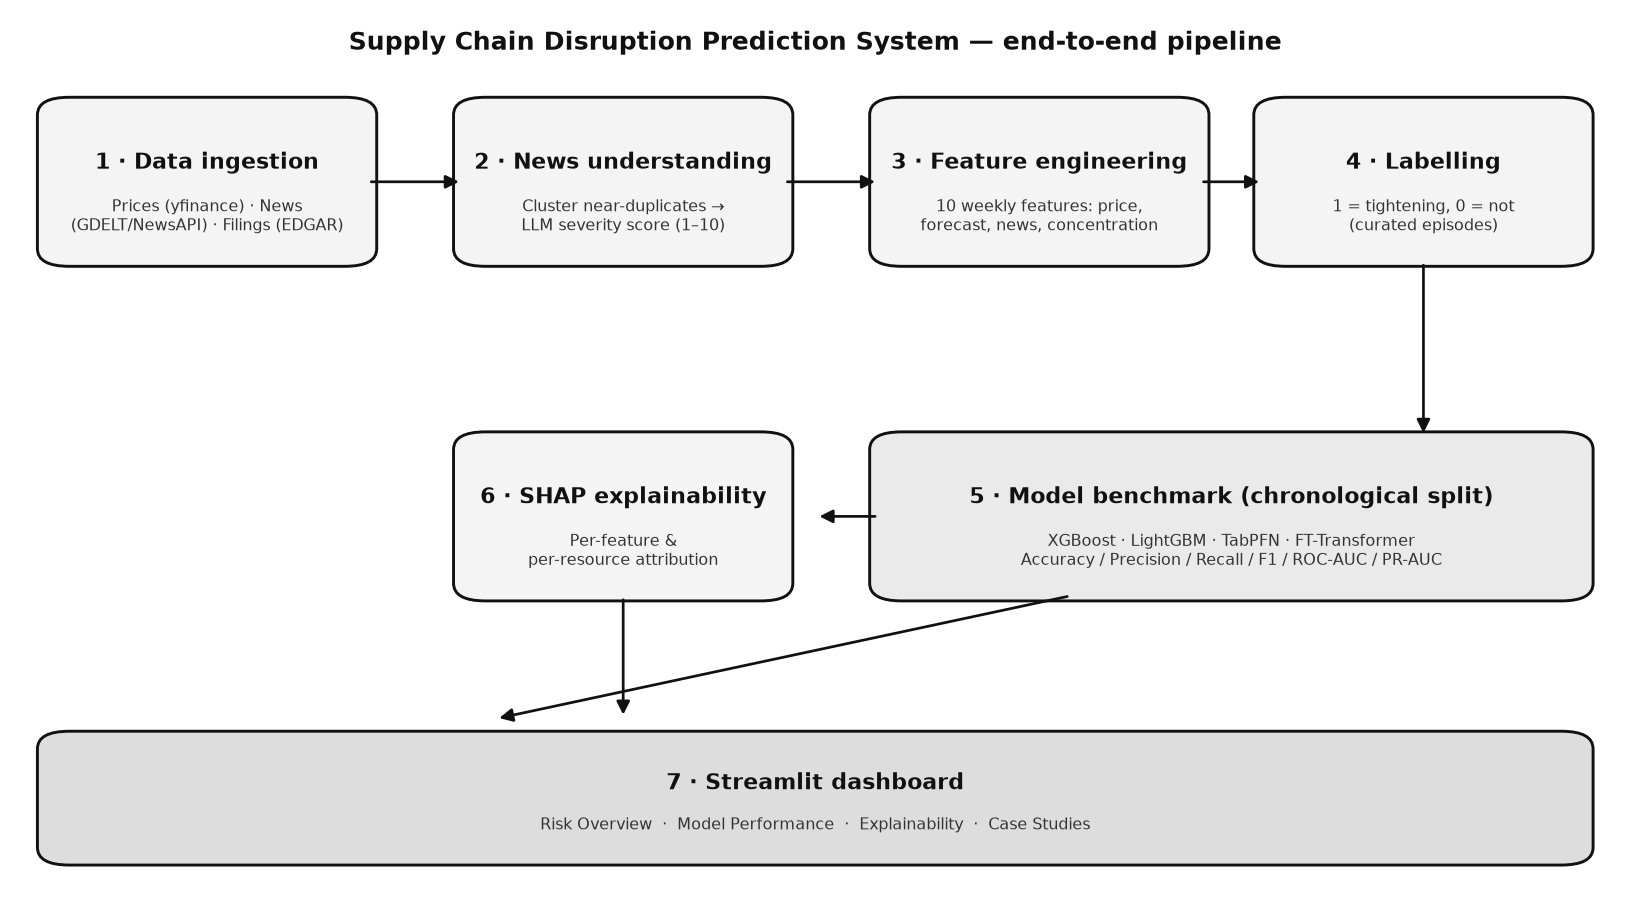
\includegraphics[width=\linewidth]{image1.png}
\caption{End-to-end architecture of the Supply Chain Disruption Prediction System.}
\end{figure}

\subsubsection{5.2.1 Data ingestion}

Producer prices (yfinance), historical and recent news (GDELT and NewsAPI) and regulatory filings (SEC EDGAR) are collected and written to a SQLite database with a normalised schema (resources, producers, price series, signals, labels and model runs).

\subsubsection{5.2.2 News understanding}

Raw news signals are clustered so that near-duplicate stories about the same event are grouped and counted once. A large language model then reads each canonical story and returns an event type and a tightening-severity score from 1 to 10. The result is a clean numeric news signal rather than free text.

\subsubsection{5.2.3 Feature engineering}

For every resource and week, the engine assembles the ten features described in Section 5.1.4. Price features capture level, momentum and abnormality; forecast features summarise a short-horizon outlook and its uncertainty; news features capture the volume and severity of coverage; and supplier concentration captures structural fragility.

\subsubsection{5.2.4 Labelling}

Weeks are labelled for tightening from hand-curated episodes and price-derived rules, giving both positive (tightening) and negative (normal) examples for supervised learning.

\subsubsection{5.2.5 Model benchmarking}

Four models --- XGBoost, LightGBM, TabPFN and FT-Transformer --- are trained on a strict chronological split: earlier weeks are used for training and the most recent weeks are held out for testing, so the model can never see the future. Every model is evaluated on the same six metrics (Accuracy, Precision, Recall, F1, ROC-AUC and PR-AUC).

\subsubsection{5.2.6 Explanation and delivery}

SHAP attributions are computed for the chosen model, both globally and per resource. Finally, an export step writes the scores, timelines, metrics, charts and attributions to files that the Streamlit dashboard reads, so the front-end stays decoupled from the engine.

% =========================================================
% 5.3 MODEL SELECTION, CONFIGURATION AND TRAINING BEHAVIOUR
% =========================================================
\subsection{5.3 Model Selection, Configuration and Training Behaviour}

Section 5.2.5 introduced the four models benchmarked by the system. This subsection examines each one individually: why it was included in the benchmark, the exact parameters and hyperparameters it was trained with, and how it actually behaved during training on the real, chronologically-split data (Section 5.1). All four models share the same ten input features (Section 5.1.4), the same chronological train/test split (Section 5.2.5), and the same random seed (42) wherever the underlying library accepts one.

\subsubsection{5.3.1 XGBoost}

\textbf{Why chosen.} XGBoost is the reference implementation of gradient-boosted decision trees and the natural starting point for a small, structured, mixed-signal tabular problem (Section 2.1). It handles missing values natively --- important here, since the forecast features are genuinely absent for many weeks --- and its \texttt{scale\_pos\_weight} parameter lets the tightening/non-tightening class imbalance be corrected for directly rather than through resampling.

\begin{longtable}[]{@{}
  >{\raggedright\arraybackslash}p{(\columnwidth - 4\tabcolsep) * \real{0.35}}
  >{\raggedright\arraybackslash}p{(\columnwidth - 4\tabcolsep) * \real{0.65}}@{}}
\toprule
\textbf{Parameter} & \textbf{Value} \\
\midrule
\endhead
\bottomrule
\endlastfoot
n\_estimators & 200 boosting rounds \\
max\_depth & 6 \\
learning\_rate & 0.1 \\
subsample & 0.8 (row subsampling per tree) \\
colsample\_bytree & 0.8 (feature subsampling per tree) \\
scale\_pos\_weight & \#negative / \#positive in the training split (corrects class imbalance) \\
eval\_metric & logloss \\
random\_state & 42 \\
\end{longtable}
\begin{center}Table 6. XGBoost parameters and hyperparameters.\end{center}

Figure 2 plots the real train and test log-loss against boosting round on the held-out chronological split. Training loss falls smoothly towards zero, while test loss levels off around round 175 --- a normal, contained overfitting gap rather than a runaway one, which is consistent with XGBoost producing the best-generalising model in the benchmark.

\begin{figure}[H]
\centering
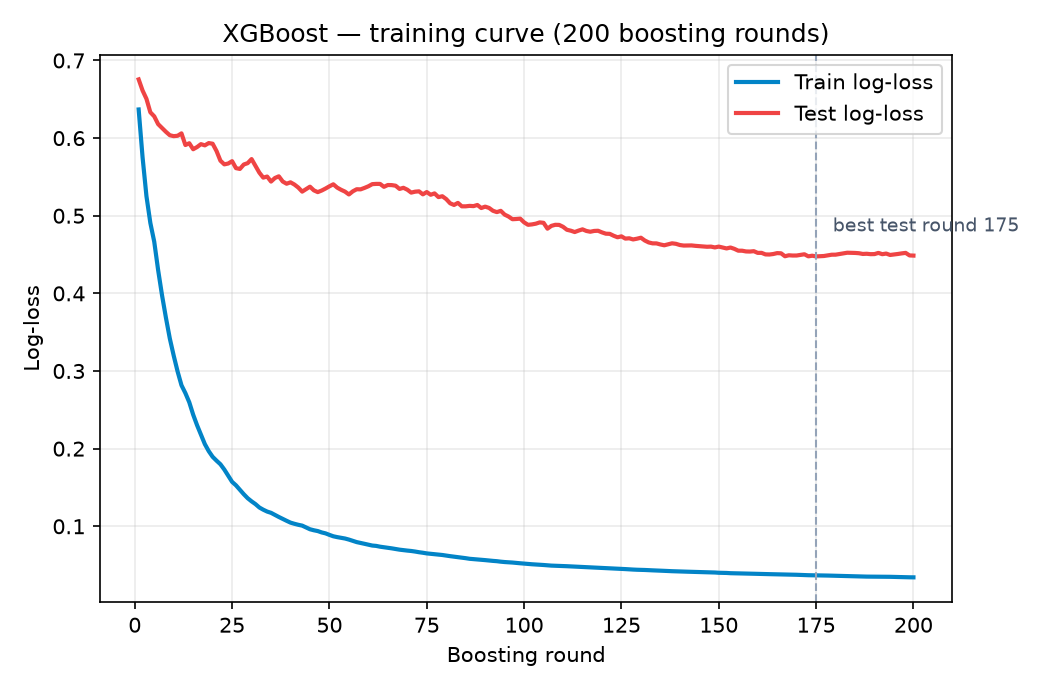
\includegraphics[width=5.4in]{model_xgboost_curve.png}
\caption{XGBoost --- real train/test log-loss versus boosting round on the chronological split.}
\end{figure}

\subsubsection{5.3.2 LightGBM}

\textbf{Why chosen.} LightGBM is a second, independent gradient-boosted-tree implementation, included as a cross-check on XGBoost rather than a duplicate of it. It grows trees leaf-wise instead of level-wise and uses histogram-based splitting, which trains an order of magnitude faster and can reach a different bias/variance trade-off on the same data --- useful for confirming whether the tree-based result is robust to implementation choices rather than an artefact of one library's defaults.

\begin{longtable}[]{@{}
  >{\raggedright\arraybackslash}p{(\columnwidth - 4\tabcolsep) * \real{0.35}}
  >{\raggedright\arraybackslash}p{(\columnwidth - 4\tabcolsep) * \real{0.65}}@{}}
\toprule
\textbf{Parameter} & \textbf{Value} \\
\midrule
\endhead
\bottomrule
\endlastfoot
n\_estimators & 100 boosting rounds \\
num\_leaves & 31 (library default) \\
max\_depth & -1, i.e. unlimited (library default) \\
learning\_rate & 0.1 (library default) \\
eval\_metric & binary\_logloss \\
random\_state & 42 \\
\end{longtable}
\begin{center}Table 7. LightGBM parameters and hyperparameters.\end{center}

Figure 3 shows a materially different picture from XGBoost: test log-loss bottoms out around round 43 and then rises steadily while training loss keeps falling --- a clear, unmitigated overfitting signature, since the fixed 100-round schedule has no early stopping to halt it at the optimum. This directly explains LightGBM's benchmark behaviour: very high precision but low recall, i.e. a model that becomes overconfident on the training distribution and correspondingly conservative at test time.

\begin{figure}[H]
\centering
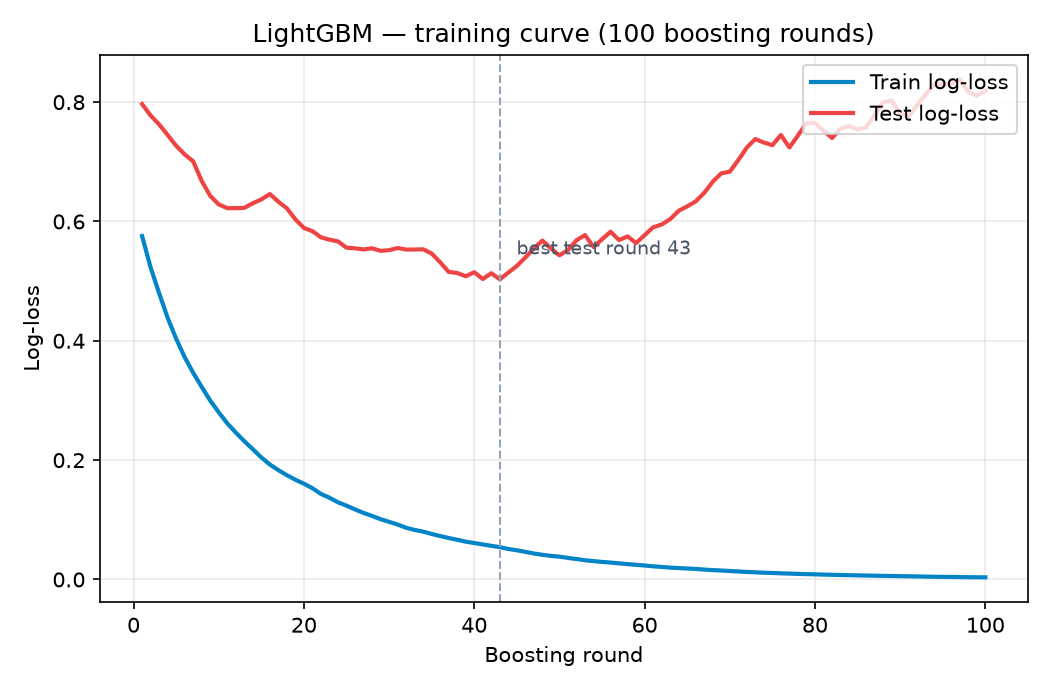
\includegraphics[width=5.4in]{model_lightgbm_curve.png}
\caption{LightGBM --- real train/test log-loss versus boosting round, run without early stopping.}
\end{figure}

\subsubsection{5.3.3 TabPFN}

\textbf{Why chosen.} TabPFN represents a fundamentally different paradigm: a transformer pre-trained once, offline, to approximate Bayesian inference over small tabular datasets, and then applied to a new dataset in a single in-context forward pass with no gradient-based training at all (Hollmann et al., 2023). It was included to test whether a modern, zero-tuning foundation model can match purpose-tuned trees on this problem --- a meaningful question given how little labelled data (Section 5.1.5) this project has to work with.

\begin{longtable}[]{@{}
  >{\raggedright\arraybackslash}p{(\columnwidth - 4\tabcolsep) * \real{0.35}}
  >{\raggedright\arraybackslash}p{(\columnwidth - 4\tabcolsep) * \real{0.65}}@{}}
\toprule
\textbf{Parameter} & \textbf{Value} \\
\midrule
\endhead
\bottomrule
\endlastfoot
Training procedure & None --- pretrained weights, in-context inference only \\
Tunable hyperparameters & None exposed by this system (library defaults) \\
Inference backend & Hosted \texttt{tabpfn-client} when a \texttt{TABPFN\_TOKEN} is configured; local gated weights otherwise \\
random\_state & Not applicable (deterministic forward pass) \\
\end{longtable}
\begin{center}Table 8. TabPFN configuration --- no hyperparameters are trained or tuned.\end{center}

Because there is no training loop, there is no loss curve to plot. Figure 4 instead shows the closest honest analogue: a reliability diagram and predicted-probability histogram computed from TabPFN's real predictions on the held-out set. The predicted probabilities are directionally well-ordered (higher predicted probability does correspond to a higher observed tightening rate) but are heavily concentrated near zero, which is consistent with TabPFN's benchmark behaviour of very high precision and very low recall --- it rarely commits to a confident positive prediction.

\begin{figure}[H]
\centering
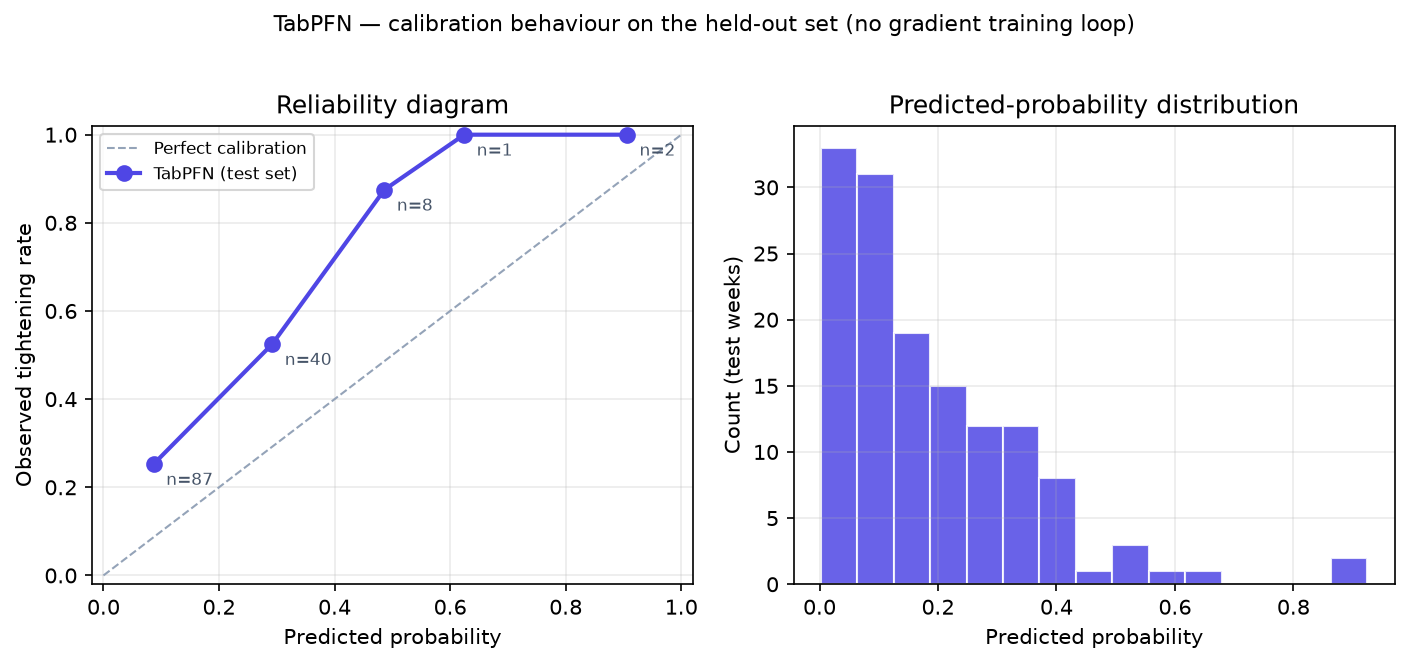
\includegraphics[width=6.0in]{model_tabpfn_curve.png}
\caption{TabPFN --- reliability diagram and predicted-probability distribution on the held-out set (no training loop exists to plot).}
\end{figure}

\subsubsection{5.3.4 FT-Transformer}

\textbf{Why chosen.} FT-Transformer is the deep-learning baseline: it tokenizes every feature and applies self-attention across them, letting the model learn feature interactions rather than have them imposed by tree splits (Gorishniy et al., 2021). It was included to test the tabular-machine-learning literature's central claim --- that deep networks need substantially more data than tree ensembles to be competitive (Grinsztajn et al., 2022) --- directly on this project's own, deliberately small dataset.

\begin{longtable}[]{@{}
  >{\raggedright\arraybackslash}p{(\columnwidth - 4\tabcolsep) * \real{0.35}}
  >{\raggedright\arraybackslash}p{(\columnwidth - 4\tabcolsep) * \real{0.65}}@{}}
\toprule
\textbf{Parameter} & \textbf{Value} \\
\midrule
\endhead
\bottomrule
\endlastfoot
dim (token embedding size) & 32 \\
depth (attention blocks) & 4 \\
heads (attention heads) & 4 \\
attn\_dropout & 0.1 \\
ff\_dropout & 0.1 \\
epochs & 30 (maximum) \\
learning\_rate & 1e-3 \\
batch\_size & 64 \\
Optimizer & Adam \\
Loss function & Binary cross-entropy with logits \\
Early stopping & Patience of 5 epochs on a held-out 10\% validation split \\
\end{longtable}
\begin{center}Table 9. FT-Transformer parameters and hyperparameters.\end{center}

Figure 5 shows the real per-epoch training curve. Validation loss rises immediately after epoch 1 while training loss continues to fall, so early stopping halts training after only 6 epochs and restores the epoch-1 weights. This is the training-level evidence for the deep model's benchmark failure (ROC-AUC below chance): with only a few hundred training weeks, FT-Transformer begins overfitting almost immediately and never reaches a useful optimum, directly confirming the literature's small-data caveat for deep tabular models (Section 2.1).

\begin{figure}[H]
\centering
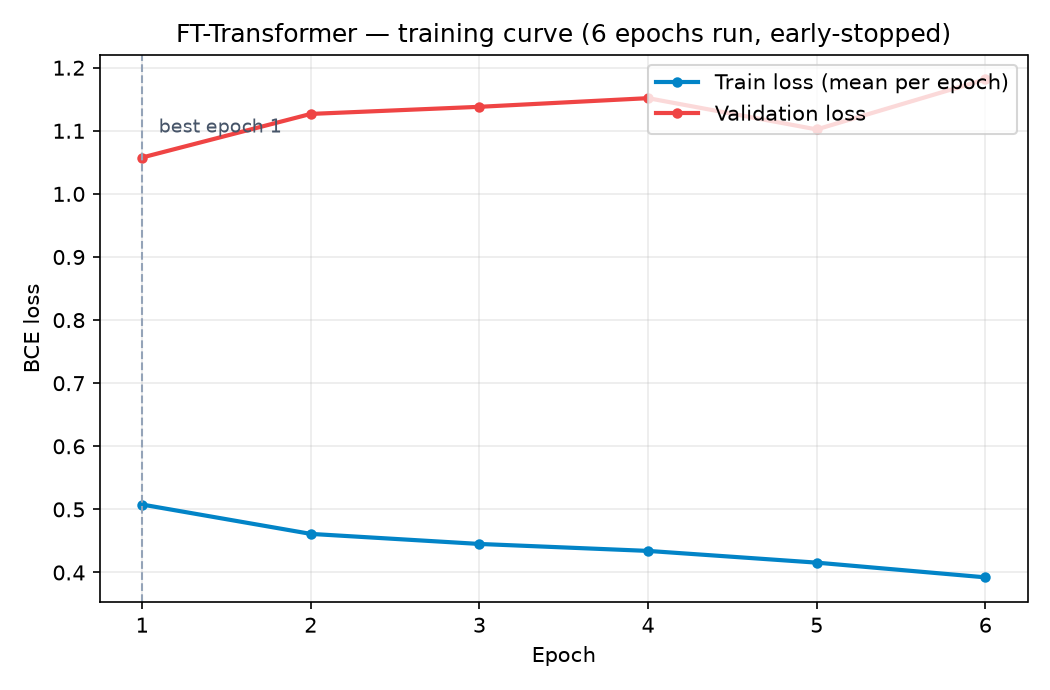
\includegraphics[width=5.4in]{model_ft_curve.png}
\caption{FT-Transformer --- real per-epoch train/validation loss; training is early-stopped after 6 epochs.}
\end{figure}

% =========================================================
% 6. RESULTS
% =========================================================
\section{6. Results}

The results below are from the latest end-to-end run. The held-out test set consists of the most recent 138 weeks, of which 53 are genuine tightening weeks (a positive base rate of 0.38). Section 5.3 examined each model individually; this section compares them head to head.

\subsection{6.1 Model benchmark}

Table 10 reports every model on the held-out set. XGBoost is the best overall model, with the highest F1 (0.71) and the strongest ranking ability (ROC-AUC 0.87). The two gradient-boosted tree models (XGBoost and LightGBM) clearly lead.

\begin{longtable}[]{@{}
  >{\raggedright\arraybackslash}p{(\columnwidth - 14\tabcolsep) * \real{0.2146}}
  >{\raggedright\arraybackslash}p{(\columnwidth - 14\tabcolsep) * \real{0.1268}}
  >{\raggedright\arraybackslash}p{(\columnwidth - 14\tabcolsep) * \real{0.1220}}
  >{\raggedright\arraybackslash}p{(\columnwidth - 14\tabcolsep) * \real{0.1122}}
  >{\raggedright\arraybackslash}p{(\columnwidth - 14\tabcolsep) * \real{0.0976}}
  >{\raggedright\arraybackslash}p{(\columnwidth - 14\tabcolsep) * \real{0.1220}}
  >{\raggedright\arraybackslash}p{(\columnwidth - 14\tabcolsep) * \real{0.1171}}
  >{\raggedright\arraybackslash}p{(\columnwidth - 14\tabcolsep) * \real{0.0878}}@{}}
\toprule
\textbf{Model} & \textbf{Accuracy} & \textbf{Precision} & \textbf{Recall} & \textbf{F1} & \textbf{ROC-AUC} & \textbf{PR-AUC} & \textbf{Time} \\
\midrule
\endhead
\bottomrule
\endlastfoot
XGBoost & 0.790 & 0.750 & 0.679 & 0.713 & 0.867 & 0.793 & 2.1s \\
LightGBM & 0.725 & 0.941 & 0.302 & 0.457 & 0.817 & 0.789 & 33.4s \\
TabPFN & 0.667 & 1.000 & 0.132 & 0.233 & 0.765 & 0.695 & 576.6s \\
FT-Transformer & 0.384 & 0.384 & 1.000 & 0.555 & 0.383 & 0.307 & 549.9s \\
\end{longtable}
\begin{center}Table 10. Model benchmark on the held-out chronological test set (best F1 in XGBoost).\end{center}

\subsection{6.2 ROC and Precision--Recall curves}

The ROC curve (Figure 6) plots true-positive rate against false-positive rate; a model that ranks well sits high and to the left, above the diagonal chance line. XGBoost and LightGBM dominate. The Precision--Recall curve (Figure 7) tells the same story against the 0.38 baseline. FT-Transformer falls below chance on both, confirming it failed to learn at this data size.

\begin{figure}[H]
\centering
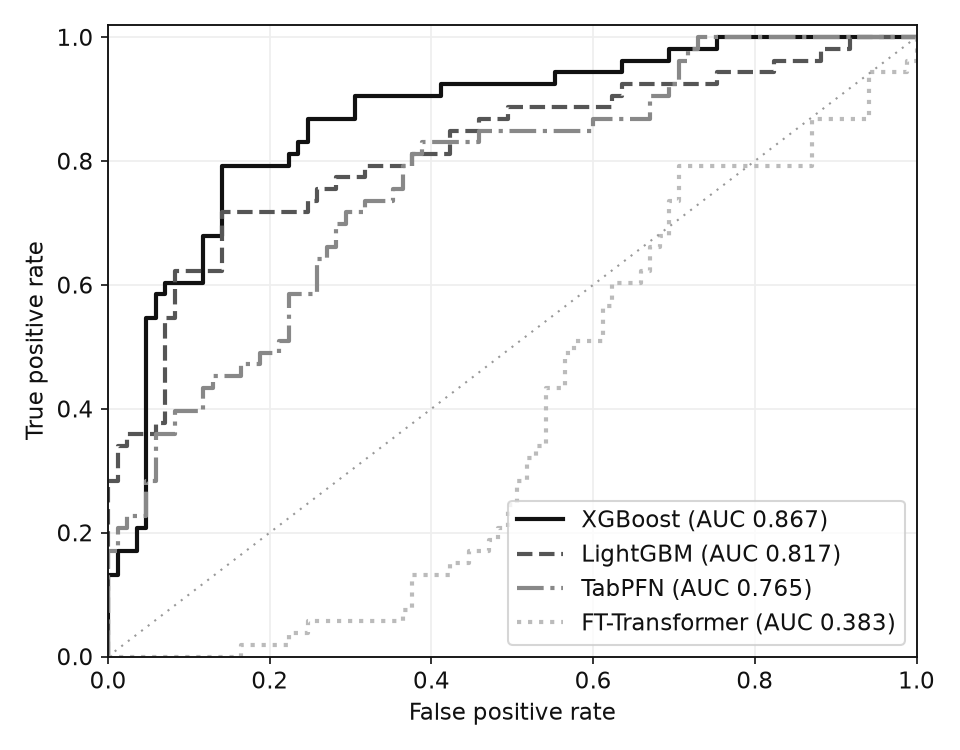
\includegraphics[width=4.47917in,height=3.5in]{image2.png}
\caption{ROC curves per model (higher and further left is better).}
\end{figure}

\begin{figure}[H]
\centering
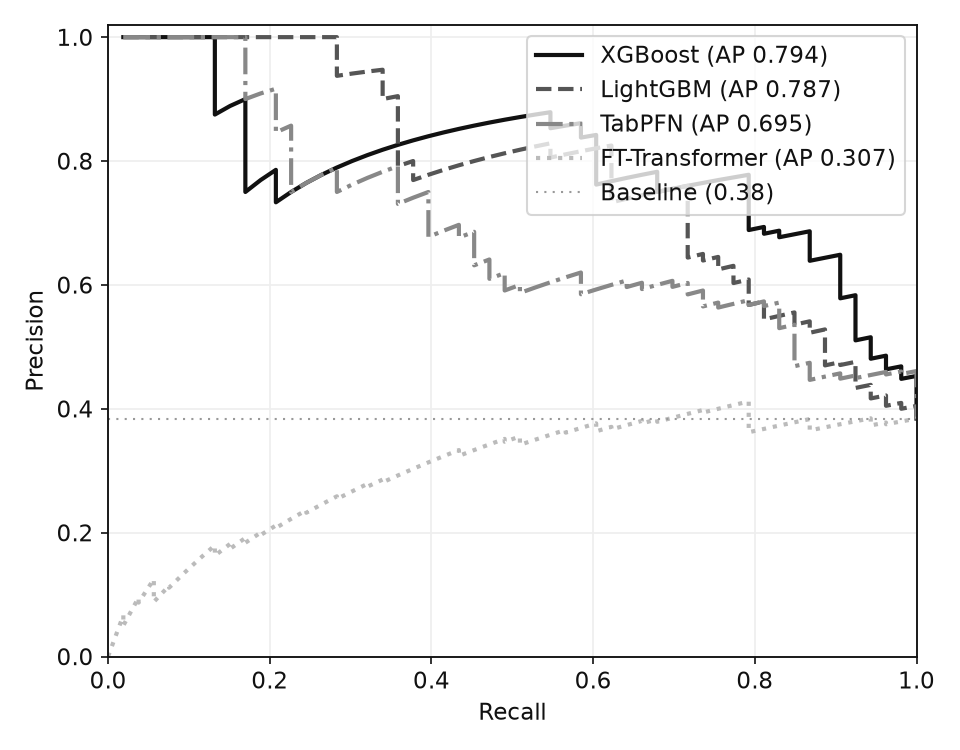
\includegraphics[width=4.47917in,height=3.5in]{image3.png}
\caption{Precision--Recall curves per model against the positive-class baseline.}
\end{figure}

\subsection{6.3 Confusion matrices}

The confusion matrices (Figure 8) reveal each model's behaviour at a 0.5 threshold. XGBoost is balanced (catches 36 of 53 tightening weeks with only 12 false alarms). LightGBM is conservative (almost no false alarms but misses most tightening). TabPFN is extremely cautious (zero false alarms, but catches only 7 of 53). FT-Transformer predicts ``risk'' for everything, which is why its accuracy collapses.

\begin{figure}[H]
\centering
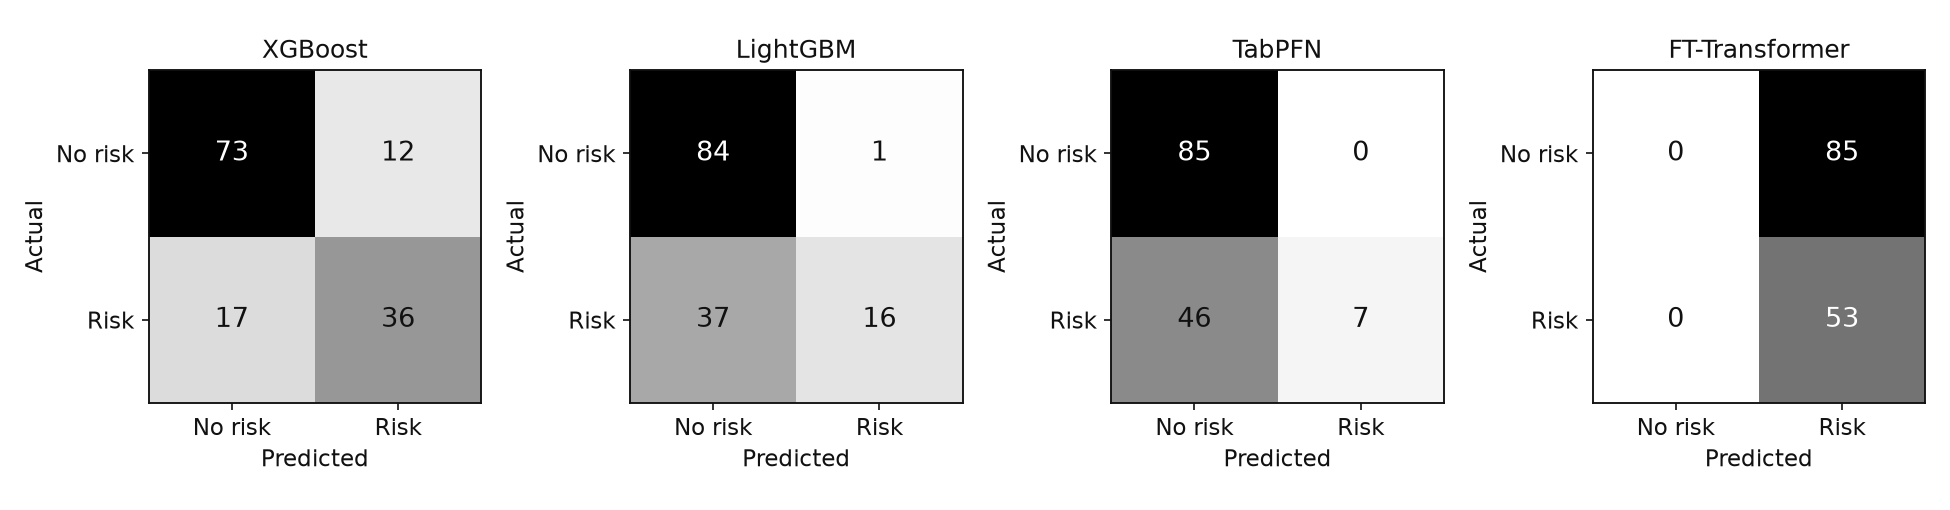
\includegraphics[width=\linewidth]{image4.png}
\caption{Confusion matrices per model (rows: actual, columns: predicted; 0.5 threshold).}
\end{figure}

\subsection{6.4 Model score timeline}

Figure 9 shows the weekly model score for all four resources, with documented tightening episodes shaded. The score rises during the episodes and falls afterwards, which is why all four resources currently read low. The score is deliberately labelled uncalibrated: it tends to saturate near 0 or 1 rather than behave as a smooth probability.

\begin{figure}[H]
\centering
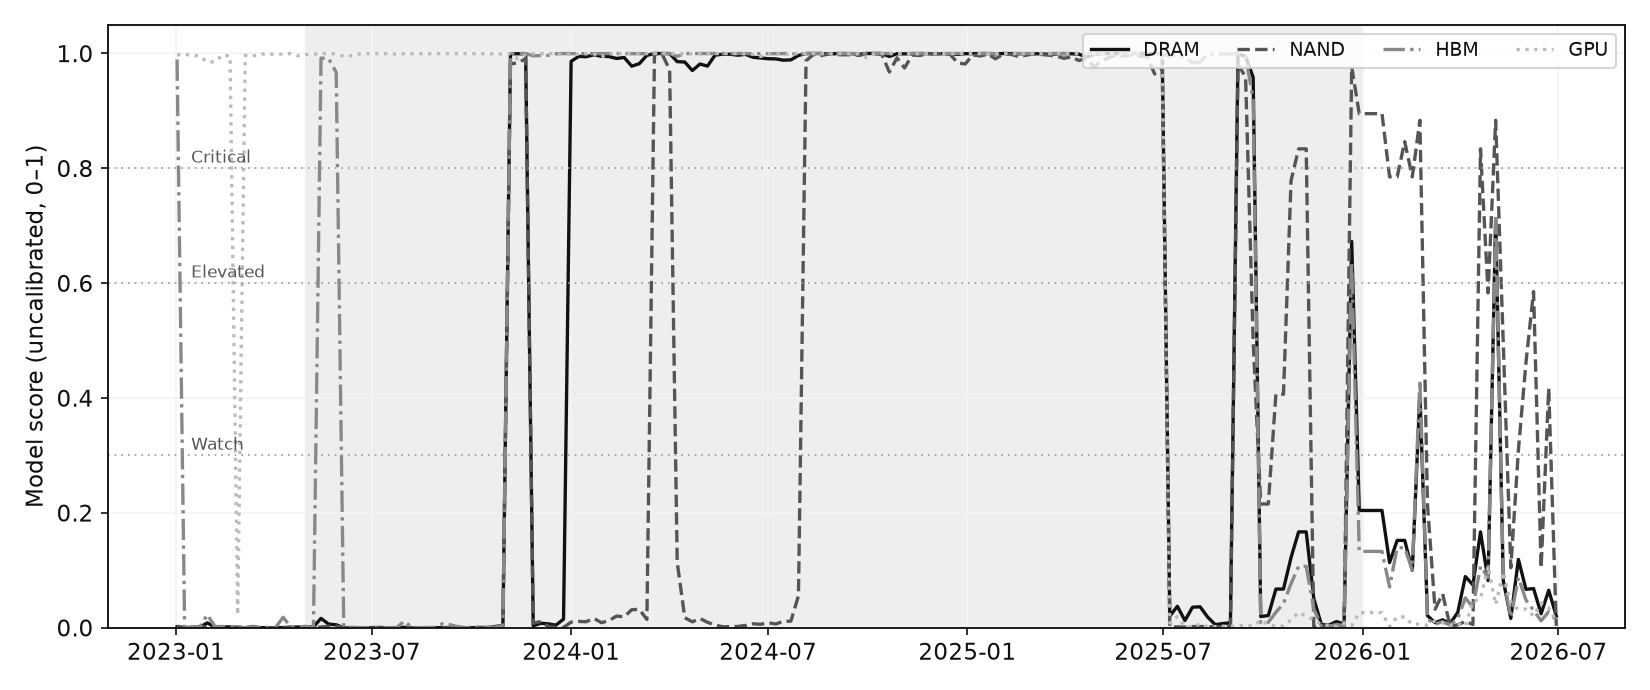
\includegraphics[width=\linewidth]{image5.png}
\caption{Weekly model score per resource, with tightening episodes shaded.}
\end{figure}

\subsection{6.5 Current risk scores}

The latest scored week (29 June 2026) yields low scores for every resource, consistent with the 2024--2025 tightening having receded:

\begin{longtable}[]{@{}
  >{\raggedright\arraybackslash}p{(\columnwidth - 4\tabcolsep) * \real{0.3421}}
  >{\raggedright\arraybackslash}p{(\columnwidth - 4\tabcolsep) * \real{0.3947}}
  >{\raggedright\arraybackslash}p{(\columnwidth - 4\tabcolsep) * \real{0.2632}}@{}}
\toprule
\textbf{Resource} & \textbf{Latest risk score} & \textbf{State} \\
\midrule
\endhead
\bottomrule
\endlastfoot
DRAM & 0.020 & Safe \\
HBM & 0.013 & Safe \\
GPU & 0.013 & Safe \\
NAND & 0.003 & Safe \\
\end{longtable}
\begin{center}Table 11. Final per-resource risk scores from the latest run.\end{center}

\subsection{6.6 Explainability}

Globally (Figure 10), the model relies most on price level, followed by supplier concentration (HHI) and price trend; news severity contributes as a supporting cue and the forecast features contribute almost nothing (and are hidden). This matches domain intuition: tightening shows up first as sustained price rises in already-concentrated markets.

\begin{figure}[H]
\centering
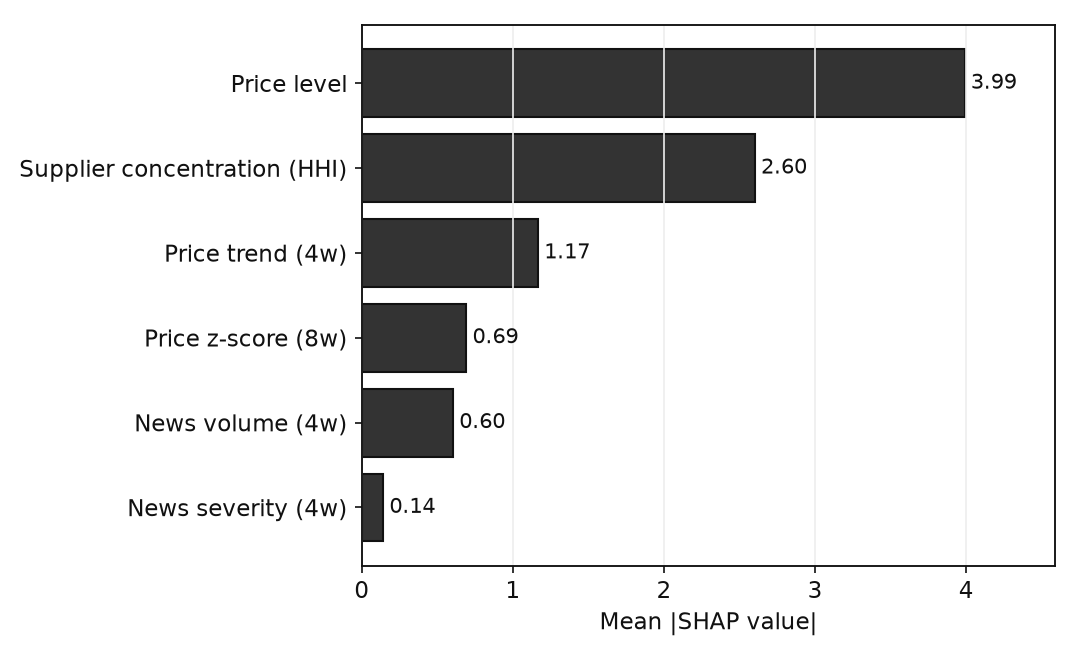
\includegraphics[width=5.41667in,height=3.3125in]{image6.png}
\caption{Global feature importance (mean absolute SHAP value).}
\end{figure}

Locally (Figure 11), the drivers for DRAM explain why it currently reads Safe: the price-level signal is a large negative (left-pointing) contribution, i.e. current prices are pulling the score down after coming off their episode peak.

\begin{figure}[H]
\centering
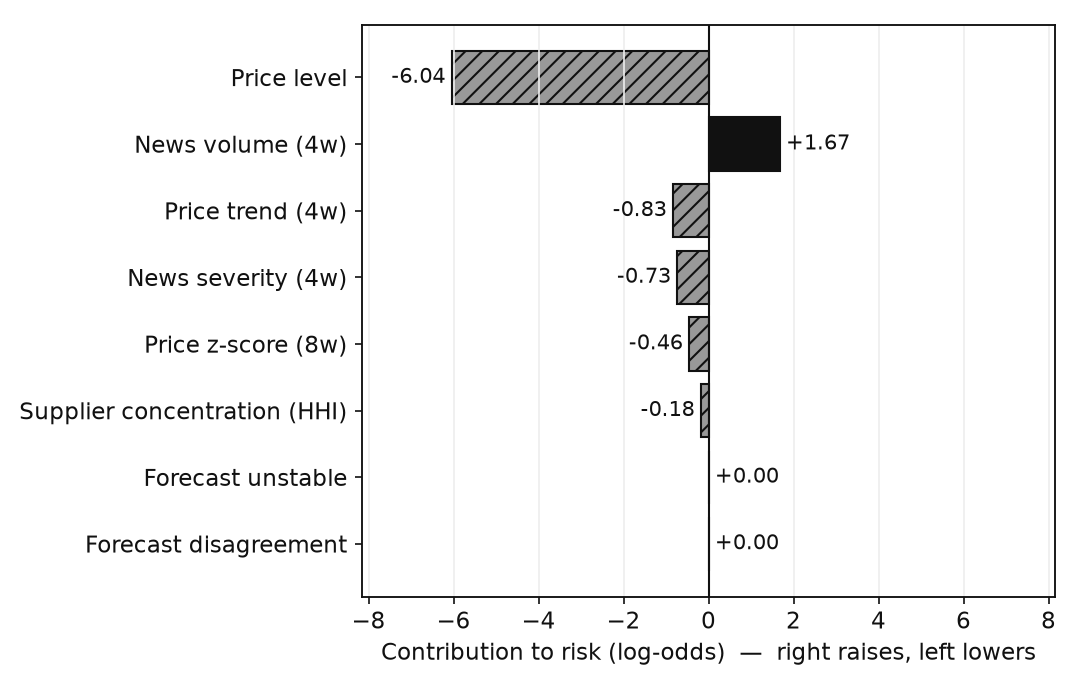
\includegraphics[width=5.41667in,height=3.45833in]{image7.png}
\caption{Per-resource SHAP drivers for DRAM (right raises risk, left lowers it).}
\end{figure}

% =========================================================
% 7. THE DASHBOARD
% =========================================================
\section{7. The Dashboard}

The Streamlit dashboard is the delivery layer. It has four pages, each reading the engine's exported files. Each page is shown below as a full-colour screenshot captured from the running application (Figures 12--15), followed by a short description of what it presents; the analytical charts these pages contain are also reproduced at full size in Section 6 (Figures 6--11).

\subsection{7.1 Risk Overview}

The landing page. It opens with an honesty note (``decision support, not certainty''), then shows a card per resource with its current score and state (Safe / Watch / Elevated / Critical), followed by the model-score timeline (Figure 9) with tightening episodes shaded, the top global risk drivers, and dataset download buttons. It answers, at a glance: how tight is each resource right now, and how did it get here.

\begin{figure}[H]
\centering
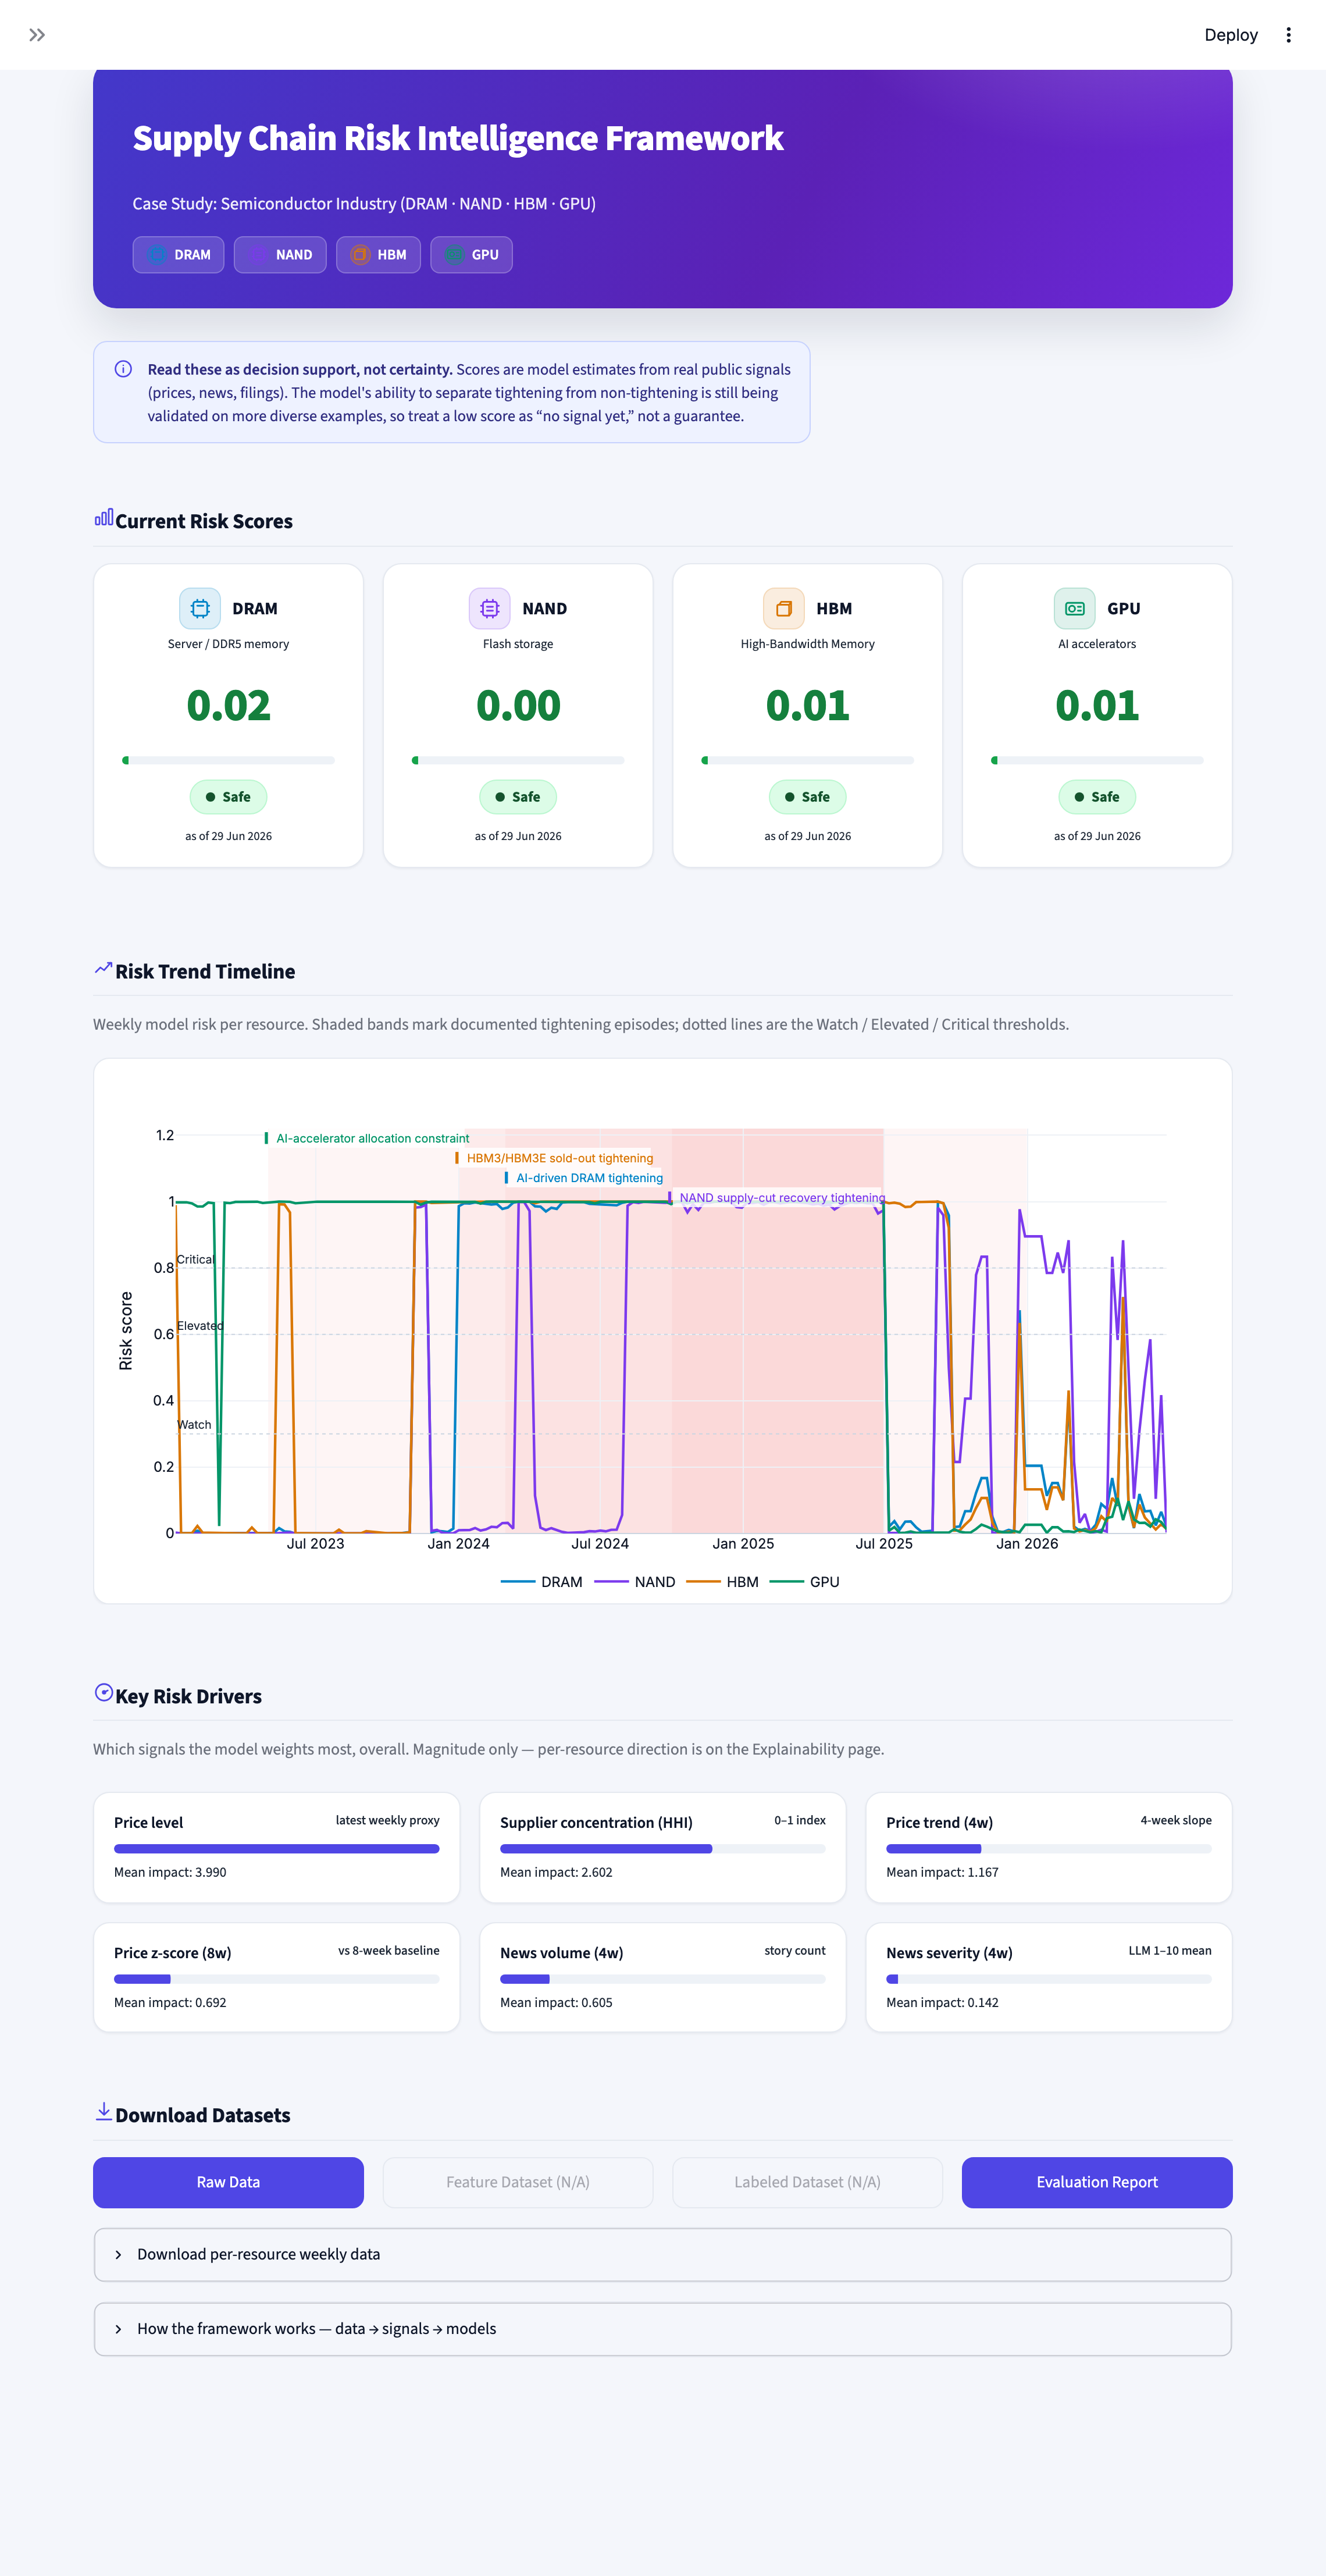
\includegraphics[width=3.91823in,height=5.85367in]{image8.png}
\caption{Dashboard --- Risk Overview page: the current risk score for each resource, the weekly risk-trend timeline with documented tightening episodes shaded, and the overall key risk drivers.}
\end{figure}

\subsection{7.2 Model Performance}

A transparency page for the benchmark. It shows the metrics table (Table 10), the ROC and Precision--Recall curves (Figures 6 and 7) and the confusion matrices (Figure 8), so a reviewer can judge not just which model was chosen but why.

\begin{figure}[H]
\centering
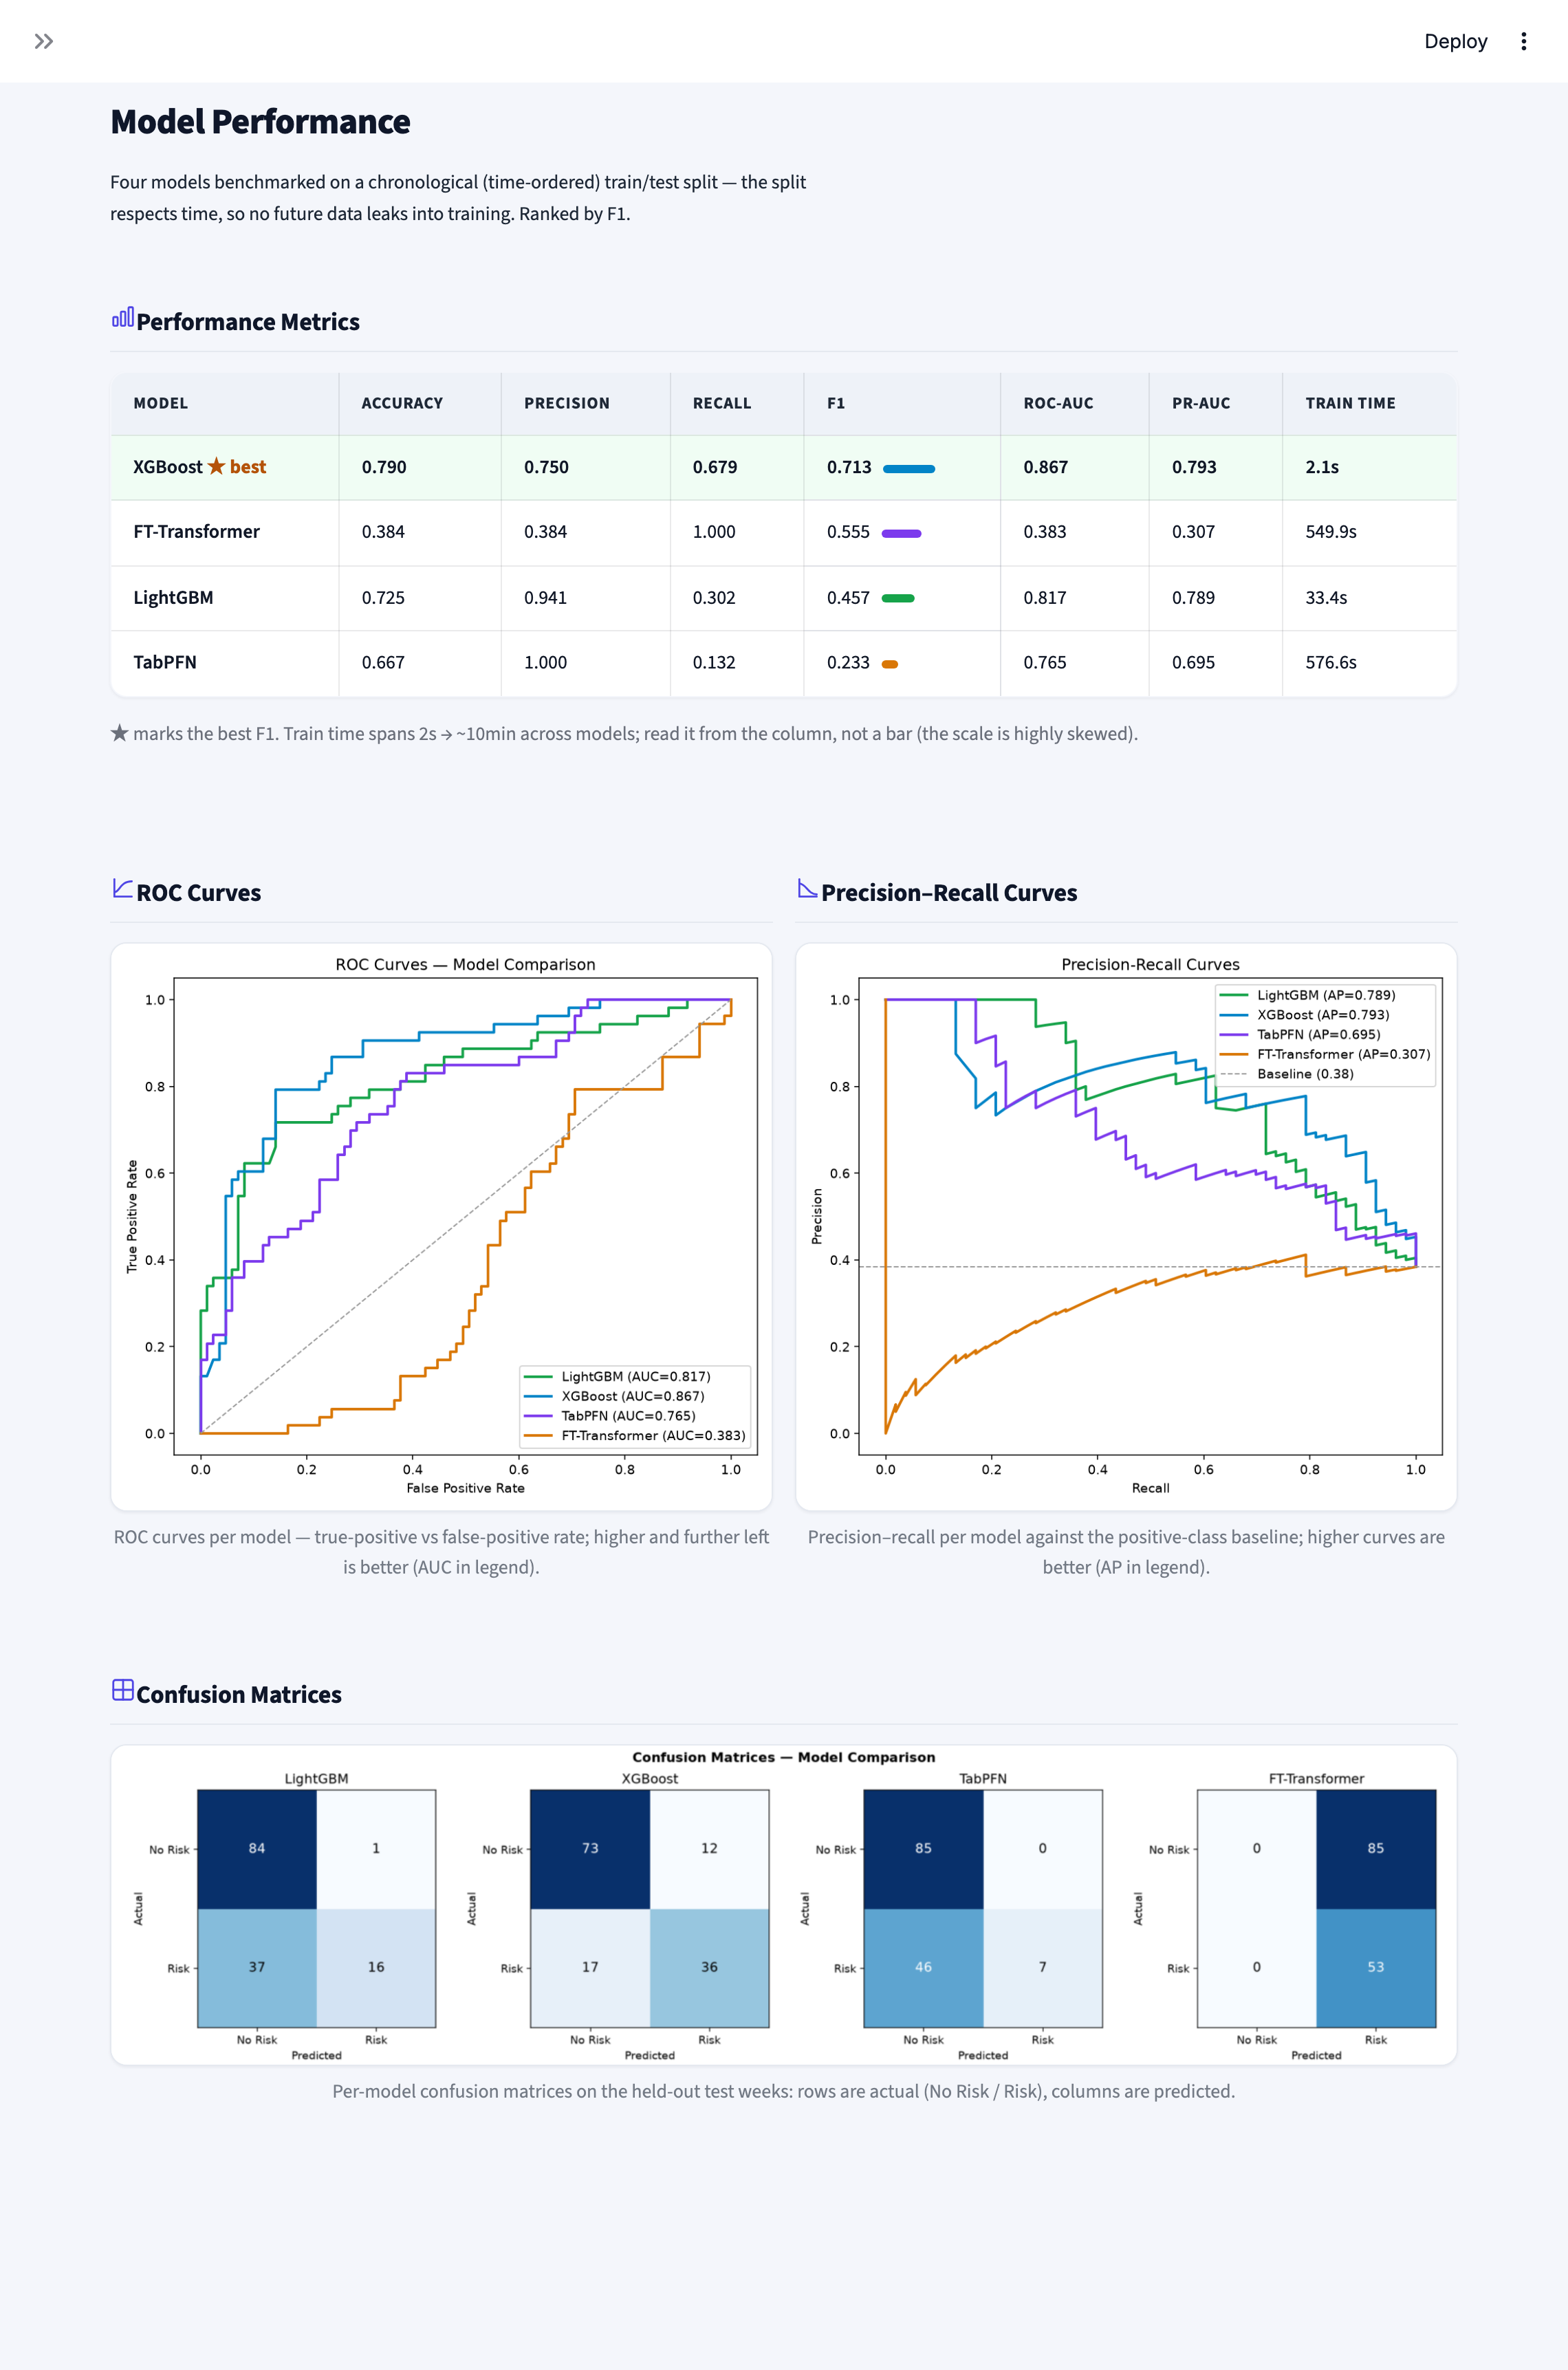
\includegraphics[width=5.02844in,height=7.6in]{image9.png}
\caption{Dashboard --- Model Performance page: the four-model benchmark metrics table, the ROC and Precision--Recall curves, and the per-model confusion matrices.}
\end{figure}

\subsection{7.3 Explainability}

Opens the model with SHAP: the global feature-importance chart (Figure 10) and a per-resource driver view (Figure 11) selectable by resource, with signed contributions (red raises risk, green lowers it).

\begin{figure}[H]
\centering
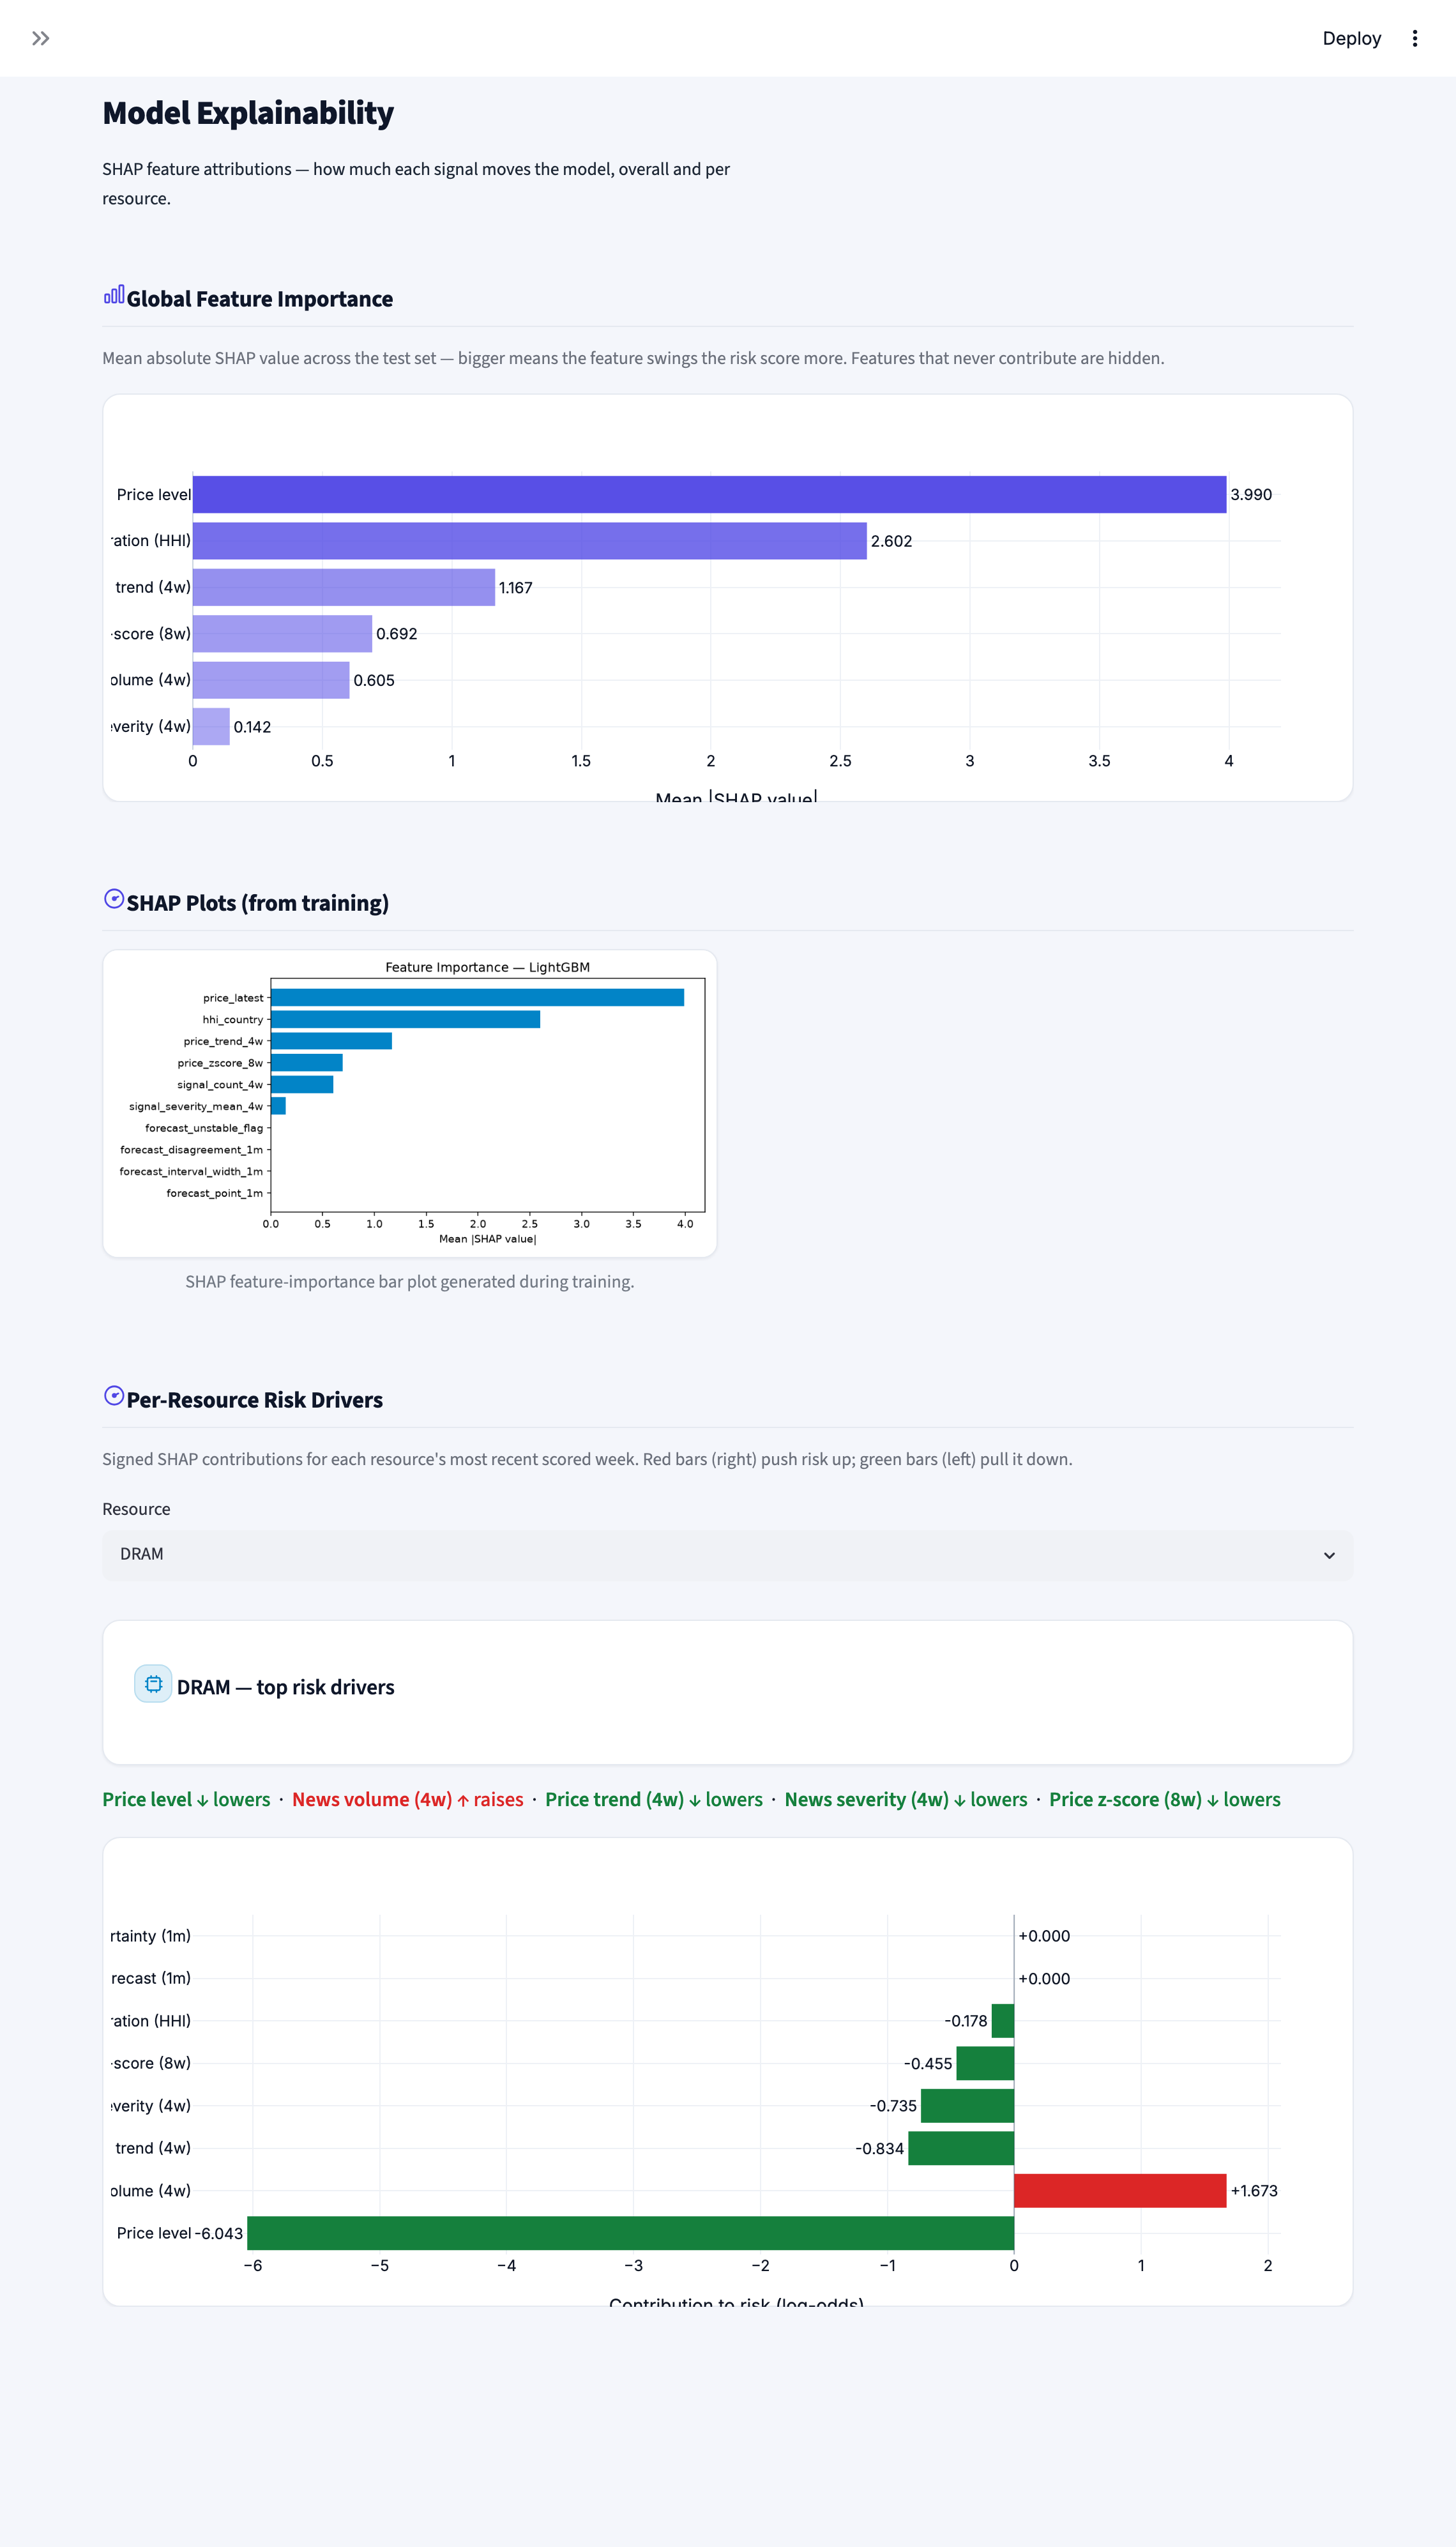
\includegraphics[width=4.34503in,height=7.6in]{image10.png}
\caption{Dashboard --- Explainability page: global SHAP feature importance and the signed per-resource risk-driver view (DRAM shown).}
\end{figure}

\subsection{7.4 Case Studies}

Documents the tightening episodes the labels are built from --- the 2024--2025 DRAM and HBM squeezes and the GPU allocation crunch --- each with its period, severity, and the qualitative indicators the engine actually tracks, overlaid on the risk timeline.

\begin{figure}[H]
\centering
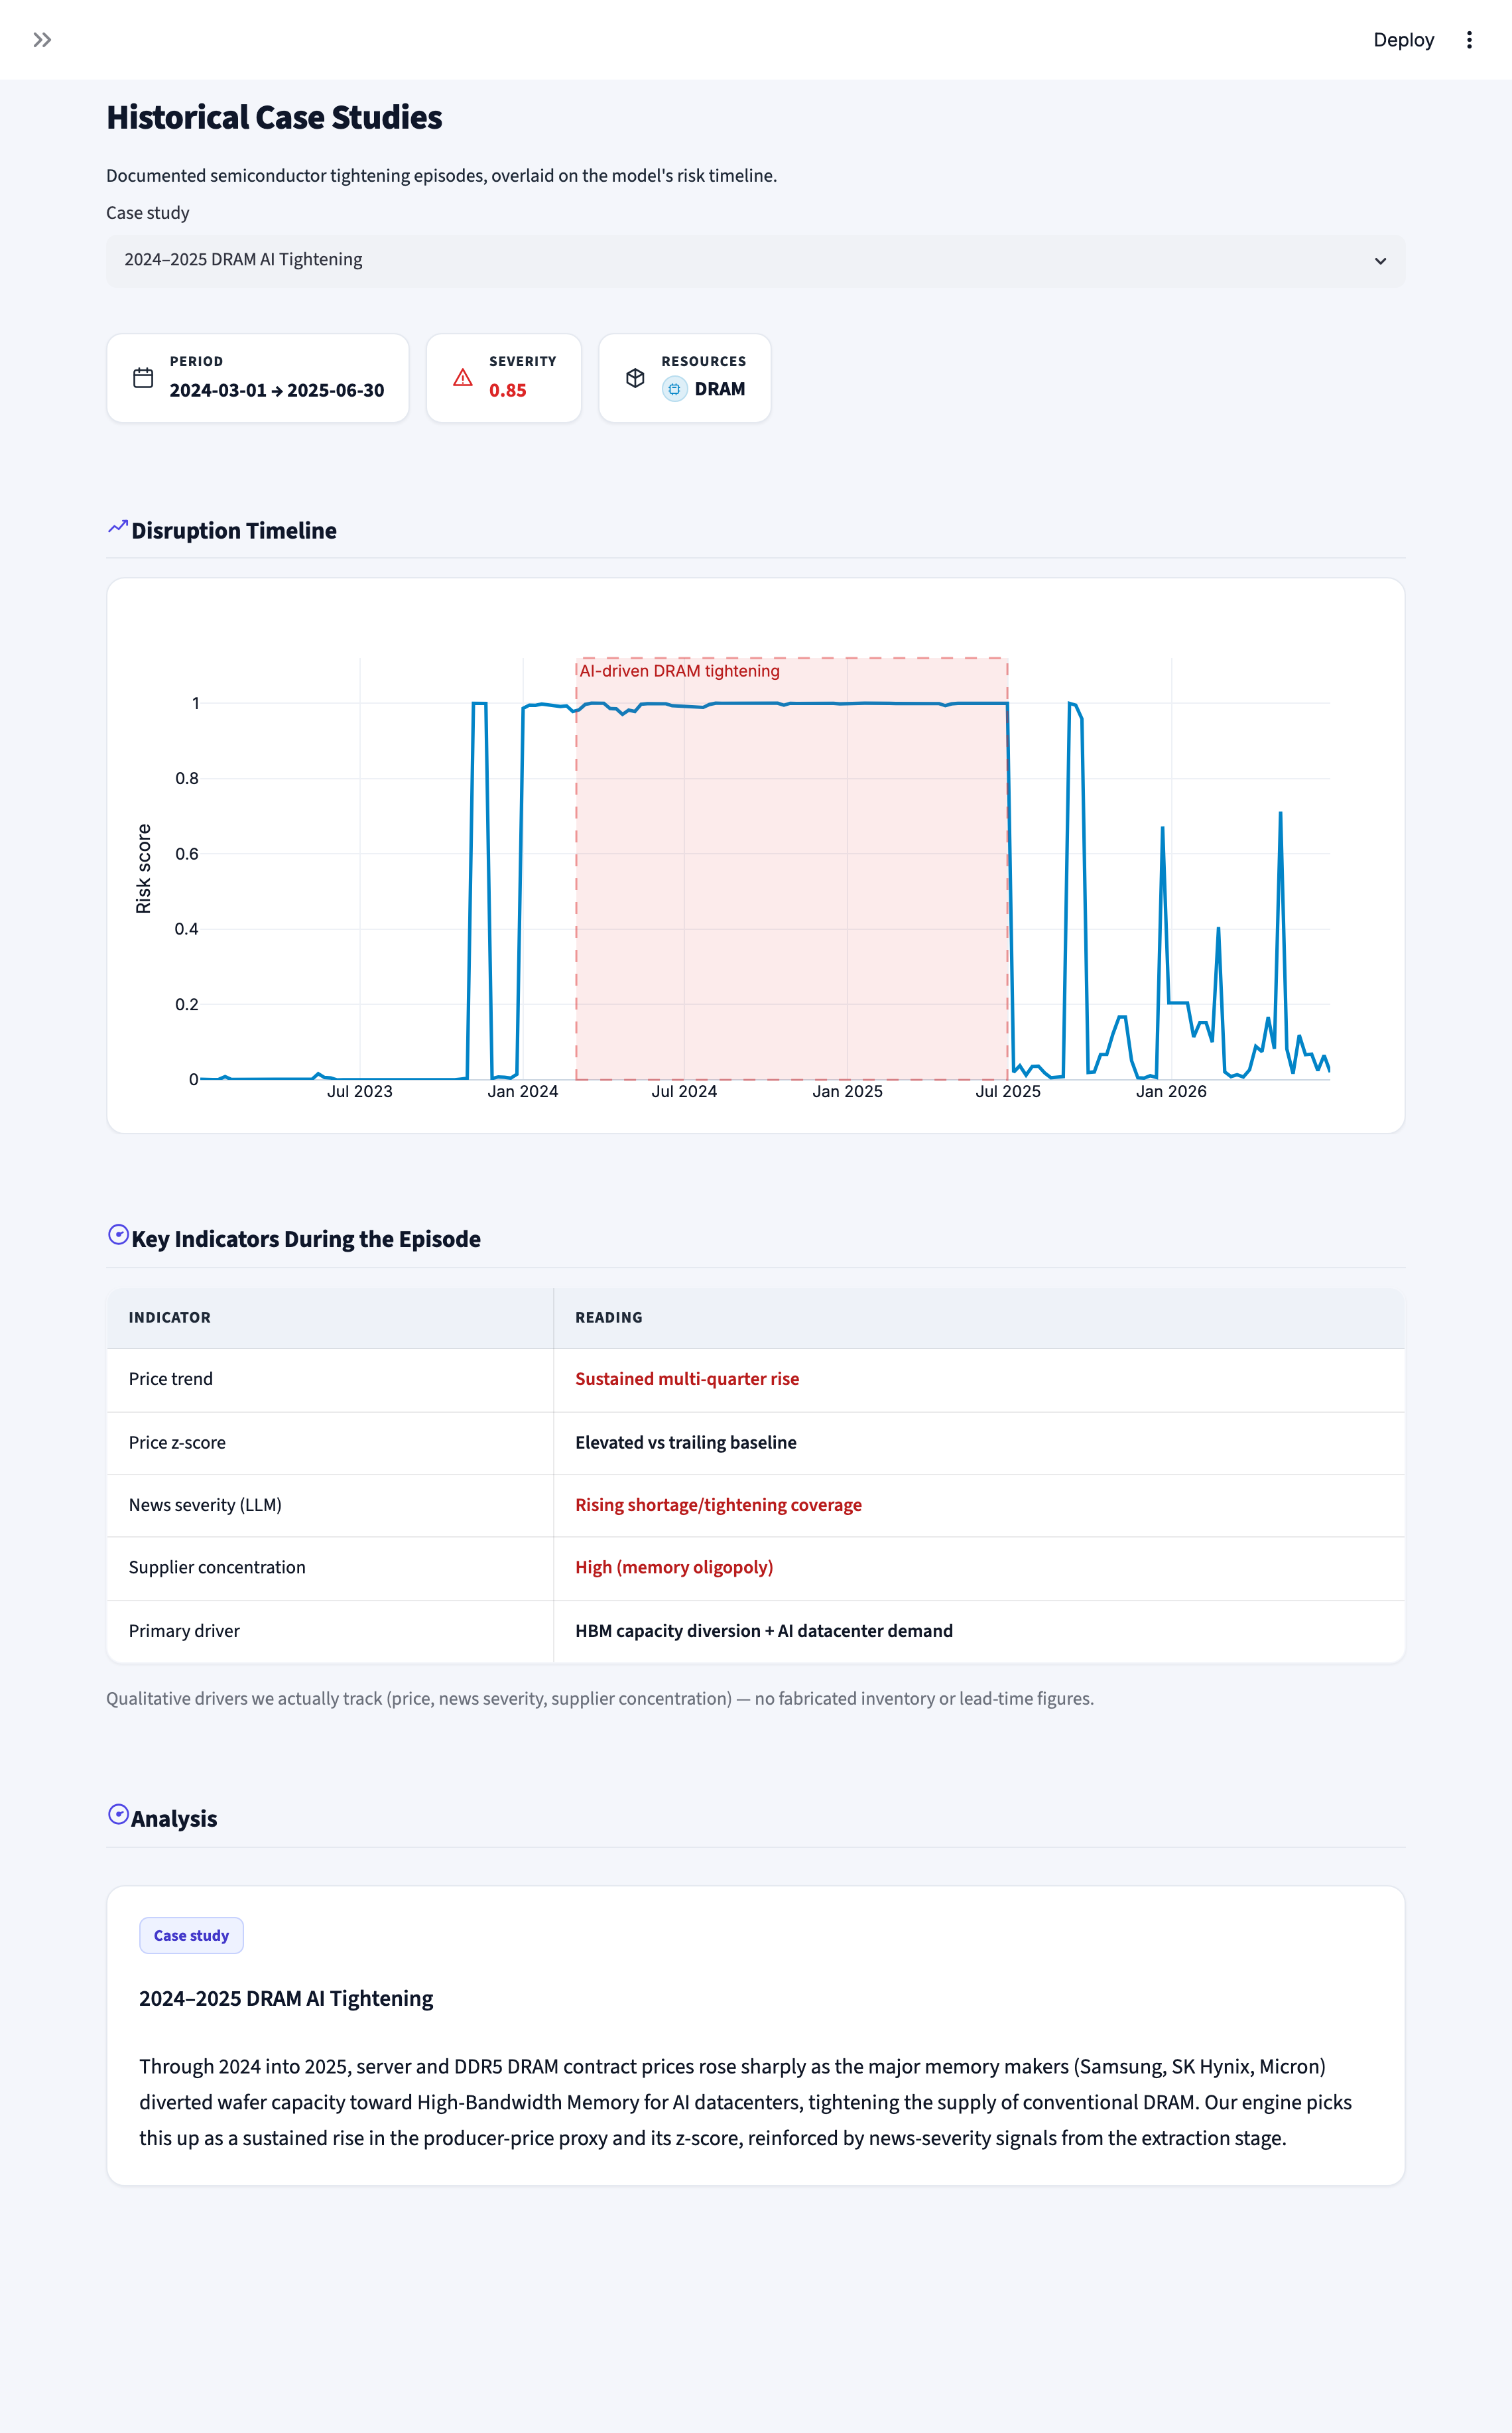
\includegraphics[width=4.7241in,height=7.6in]{image11.png}
\caption{Dashboard --- Case Studies page: the documented tightening episodes the training labels are built from.}
\end{figure}

% =========================================================
% 8. LIMITATIONS
% =========================================================
\section{8. Limitations}

The system is a working prototype and its results should be read with the following limitations in mind:

\begin{itemize}[topsep=4pt]
\item Time-confounded negatives. The non-tightening examples are concentrated in the 2023 memory glut, so the chronological split partly separates by time period. The model ranks tightening weeks well (AUC $\approx$ 0.87) but this figure may be optimistic.
\item Uncalibrated score. The raw model score saturates near 0 or 1 and is not a calibrated probability. It is best read as ``does this week resemble a known tightening window?'' rather than ``the probability of tightening is X\%.''
\item Data recency and coverage. Scores are only as fresh as the latest scored week, and the price signal is a market proxy rather than direct contract pricing.
\item Small data for deep models. With only a few hundred training weeks, the deep FT-Transformer underfits; the system therefore relies on gradient-boosted trees.
\item Label subjectivity. Tightening episodes are partly hand-curated, which introduces some subjectivity into the ground truth.
\end{itemize}

The clearest next step is to broaden the negative examples across more time periods so that discrimination can be validated on genuinely diverse data, and then to calibrate the score into a true probability.

% =========================================================
% 9. CONCLUSION
% =========================================================
\section{9. Conclusion}

This project delivers a complete, working early-warning system for semiconductor supply tightening across DRAM, NAND, HBM and GPUs. It fuses real public signals --- prices, news and filings --- into ten weekly features per resource, uses a large language model to turn news into a numeric severity signal, benchmarks four machine-learning models on an honest chronological split, explains every prediction with SHAP, and presents the result in a clear four-page dashboard.

The headline result is that gradient-boosted trees, and XGBoost in particular, rank tightening weeks well (ROC-AUC $\approx$ 0.87), consistent with the tabular-machine-learning literature and confirmed by a benchmark that also tested a tabular foundation model and a deep network. The system is deliberately honest about its main limitation --- a time-confounded, uncalibrated score --- and builds that caveat into the interface. With broader negative data and score calibration, the framework provides a solid, extensible foundation for operational supply-risk monitoring.

% =========================================================
% REFERENCES
% =========================================================
\section*{References}
\addcontentsline{toc}{section}{References}

\begin{itemize}[leftmargin=0pt, itemindent=1.5em, topsep=4pt, itemsep=6pt]
\item[] Araci, D. (2019). FinBERT: Financial Sentiment Analysis with Pre-trained Language Models. arXiv:1908.10063.
\item[] Baryannis, G., Validi, S., Dani, S., and Antoniou, G. (2019). Supply chain risk management and artificial intelligence: state of the art and future research directions. International Journal of Production Research, 57(7).
\item[] Chen, T., and Guestrin, C. (2016). XGBoost: A Scalable Tree Boosting System. Proceedings of KDD 2016.
\item[] Gorishniy, Y., Rubachev, I., Khrulkov, V., and Babenko, A. (2021). Revisiting Deep Learning Models for Tabular Data. NeurIPS 2021.
\item[] Grinsztajn, L., Oyallon, E., and Varoquaux, G. (2022). Why do tree-based models still outperform deep learning on tabular data? NeurIPS 2022.
\item[] Hollmann, N., M\"uller, S., Eggensperger, K., and Hutter, F. (2023). TabPFN: A Transformer That Solves Small Tabular Classification Problems in a Second. ICLR 2023.
\item[] Ke, G., Meng, Q., Finley, T., et al. (2017). LightGBM: A Highly Efficient Gradient Boosting Decision Tree. NeurIPS 2017.
\item[] Leetaru, K., and Schrodt, P. A. (2013). GDELT: Global Data on Events, Location and Tone. International Studies Association Annual Convention.
\item[] Lundberg, S. M., and Lee, S.-I. (2017). A Unified Approach to Interpreting Model Predictions (SHAP). NeurIPS 2017.
\item[] Shwartz-Ziv, R., and Armon, A. (2022). Tabular Data: Deep Learning is Not All You Need. Information Fusion, 81.
\end{itemize}

\end{document}
